%
% Tex input file for CGIO User's Guide
%
% To generate a DVI file, then a PostScript file named midlevel.ps:
%
%     latex cgio.tex
%     dvips cgio.dvi -o
%
% To generate a PDF file named cgio.pdf:
%
%     pdflatex cgio.tex


\documentclass[twoside,fleqn]{article}

%
% Packages
%
%\usepackage{times}			% use PostScript Times-Roman for text
\usepackage{indentfirst}		% indent first paragraph in sections
%\usepackage[first,light]{draftcopy}	% add DRAFT watermark
\usepackage[tbtags]{amsmath}		% use ams math package
\usepackage{graphicx}			% for including eps files
%\usepackage{subfigure}			% for sub-figures
\usepackage[bf]{caption}		% for more flexible captions
   \setlength{\captionmargin}{18pt}	% caption margins
\usepackage{array}			% use new array and table package
   \setlength{\extrarowheight}{2pt}	% increase row heights in tables
\usepackage{tabularx}			% use tabularx package
\usepackage{longtable}			% use longtable package
\usepackage{alltt}			% verbatim input with font changes
%\usepackage{lscape}			% for landscape pages
%\usepackage{mdwtab}			% use mdwtab array and table package
%\usepackage{tabls}			% access \hline[dimen] feature
%\usepackage{dcolumn}			% allow table alignment at dec points
%   \newcolumntype{d}[1]{D{.}{.}{#1}}	% for tables, arg is # decimal places
\usepackage{natbib}			% for author-year citations
   \setlength{\bibhang}{0pt}		% don't use hanging indent format
\usepackage[normalem]{ulem}		% allow underlining
\usepackage{calc}			% calculation package
\usepackage{ifthen}			% control structures
\usepackage{fancyhdr}			% fancy headers and footers
   \fancyhf{}
   \renewcommand{\headrulewidth}{0pt}
   \renewcommand{\footrulewidth}{0pt}
\usepackage{titling}			% more title page control
\usepackage{xspace}			% common-sense spacing after text macro
\usepackage{mdwlist}			% more flexible description lists
\usepackage{colortbl}			% colored table cells
\usepackage{color}			% colors and grays
   \definecolor{subcolor}{rgb}{0.808,0.851,1.0}
   \definecolor{input}{rgb}{0.200,0.200,1.0}
   \definecolor{output}{rgb}{0.600,0.0,0.0}
\usepackage{url}			% typesetting urls
   \urlstyle{rm}
%\usepackage[T1]{fontenc}		% for better-looking "_" and tt "{"
\usepackage{ae}				% used instead of above for PDF output
\usepackage{hyperref}			% for hypertext links in PDF
   \hypersetup{letterpaper,plainpages=false,
               pdftitle={CGIO Users's Guide},
               pdfauthor={CGNS Project Group},
               colorlinks,
               linkcolor=blue,citecolor=blue,filecolor=red,pagecolor=blue,
               urlcolor=red}
   \renewcommand{\sectionautorefname}{Section}
   \renewcommand{\subsectionautorefname}{Section}
   \renewcommand{\subsubsectionautorefname}{Section}

%
% Page layout
%
\normalsize
\setlength{\oddsidemargin}{0.5in}	% left margins-1.0in for odd/even pages
\setlength{\evensidemargin}{0.0in}
\setlength{\textwidth}{6.0in}		% text width
%\setlength{\marginparwidth}{0in}	% margin note space parameters
%\setlength{\marginparsep}{0in}
%\setlength{\oddsidemargin}{0.25in}	% left margins-1.0in for odd/even pages
%\setlength{\evensidemargin}{0.75in}
%\setlength{\textwidth}{5.5in}		% text width
\setlength{\marginparwidth}{1.1in}	% margin note space parameters
\setlength{\marginparsep}{0.2in}
\reversemarginpar
\setlength{\topmargin}{-0.5in}		% top margin-1.0in
\setlength{\headheight}{0.25in}		% header space parameters
\setlength{\headsep}{0.5in}
\setlength{\textheight}{8.5in}		% text height
\setlength{\topskip}{\baselineskip}	% dist from top of body to 1st baseline
\setlength{\footskip}{0.75in}		% dist from bottom of body to footer
\raggedbottom				% to avoid stretching vertical space
\pagestyle{fancy}			% using fancyhdr package
\fancypagestyle{plain}{%		% page # in corner for plain style
   \fancyhf{}
   \fancyfoot[LE,RO]{\bfseries \thepage}}

%
% Misc spacing parameters
%
%\setlength{\parskip}{\baselineskip}	% blank space between paragraphs
\setlength{\parskip}{0.5\baselineskip}	% blank space between paragraphs
\setlength{\doublerulesep}{0pt}		% for wider \hlines
\setlength{\fboxsep}{5pt}		% for more margin in boxes
\newlength{\saveparindent}		% save for use where LaTeX changes them
\newlength{\saveparskip}		% save for use where LaTeX changes them
\newlength{\savebaselineskip}
\setlength{\saveparindent}{\parindent}
\setlength{\saveparskip}{\parskip}
\setlength{\savebaselineskip}{\baselineskip}
\newlength{\tmplength}			% for temp use wherever needed
\newlength{\Pwidth}			% for use in tables
\newlength{\Pwidtha}

%
% User-defined environments
%
% "Definition" list with variable-length entries, indented. Requires
% mdwlist package. (See LaTeX Companion, p 64, and mdwlist documentation.)
\newenvironment{Ventryi}[1]%
   {\settowidth{\tmplength}{\hspace{\saveparindent}#1\hspace{1em}}%
    \begin{basedescript}{%
           \desclabelwidth{\tmplength}%
           \desclabelstyle{\nextlinelabel}%
           \renewcommand{\makelabel}[1]{\hspace{\saveparindent}##1\hfil}}}
   {\end{basedescript}}
% Indented definition list with variable-length entries, compact. Requires
% mdwlist package. (See LaTeX Companion, p 64, and mdwlist documentation.)
\newenvironment{Ventryic}[1]%
   {\settowidth{\tmplength}{\hspace{\saveparindent}#1\hspace{1em}}%
    \begin{basedescript}{%
           \desclabelwidth{\tmplength}%
           \desclabelstyle{\nextlinelabel}%
           \renewcommand{\makelabel}[1]{\hspace{\saveparindent}##1\hfil}
           \setlength{\topsep}{0in}%
           \setlength{\parsep}{0in}%
           \setlength{\itemsep}{0in}}}
   {\end{basedescript}}

% "changes" environment, to identify changed code by color.  The color is
% given by the argument, with a default of red.  When the environment is
% exited, the color is changed to black.
\newenvironment{changes}[1][red]%
   {\color{#1}}
   {\color{black}}

% Adapted from comp.text.tex post by Keith Reckdahl
% (reckdahl@am-sparc7.Stanford.EDU)
% Indents text from the left margin by current value of the list
% length \leftmargin
%\newenvironment{indleft}%
%   {\begin{list}{}
%      {\setlength{\topsep}{0pt}%
%       \setlength{\listparindent}{0pt}%
%       \setlength{\itemindent}{0pt}%
%       \setlength{\parsep}{\parskip}%
%      }%
%      \item[]}%
%   {\end{list}}
% As above, but surrounding an alltt environment
\newenvironment{indlefttt}%
   {\begin{list}{}
      {\setlength{\topsep}{0pt}%
       \setlength{\listparindent}{0pt}%
       \setlength{\itemindent}{0pt}%
       \setlength{\parsep}{\parskip}%
      }%
      \item[]%
      \begin{alltt}}%
   {\end{alltt}\end{list}}
%
% Framed box for function syntax
% Works
%\newlength{\Headwidtha}
%\newlength{\savearrayrulewidth}
%\newenvironment{fctbox}
%   {\noindent
%    \setlength{\savearrayrulewidth}{\arrayrulewidth}%
%    \setlength{\arrayrulewidth}{0.6pt}%
%    \setlength{\Headwidtha}{\textwidth-3\arrayrulewidth-4\tabcolsep-0.45in}%
%    \setlength{\tmplength}{\tabcolsep+0.3in}%
%    \begin{flushleft}
%    \begin{tabular}{|>{\ttfamily\columncolor{subcolor}}p{\Headwidtha} |%
%	  >{\centering\ttfamily\columncolor{subcolor}[\tabcolsep][\tmplength]}p{0.15in}%
%	  @{\centering}p{0.15in} @{\centering}p{0.15in} |}%
%    \hline
%    \textnormal{\textbf{Functions}} & \textnormal{\textbf{Modes}} & & \\
%    \hline
%   }
%   {\hline
%    \end{tabular}
%    \setlength{\arrayrulewidth}{\savearrayrulewidth}%
%    \end{flushleft}
%   }

% 
\newlength{\Headwidtha}
\newlength{\savearrayrulewidth}
\newenvironment{fctbox}
   {\noindent
    \setlength{\savearrayrulewidth}{\arrayrulewidth}%
    \setlength{\arrayrulewidth}{0.8pt}%
    \settowidth{\tmplength}{\textbf{Modes}}
    \setlength{\Headwidtha}{\textwidth-3\arrayrulewidth-4\tabcolsep-\tmplength}%
    \begin{flushleft}
    \begin{tabular}{|>{\ttfamily\columncolor{subcolor}}p{\Headwidtha}%
                    |>{\ttfamily\columncolor{subcolor}}c |}
    \hline
    \textnormal{\textbf{Functions}} & \textnormal{\textbf{Modes}} \\
    \hline
   }
   {\hline
    \end{tabular}
    \setlength{\arrayrulewidth}{\savearrayrulewidth}%
    \end{flushleft}
   }

% Doesn't work ...
%\newlength{\Headwidtha}
%\newlength{\savearrayrulewidth}
%\newenvironment{fctbox}
%   {\noindent
%    \setlength{\savearrayrulewidth}{\arrayrulewidth}%
%    \setlength{\arrayrulewidth}{0.6pt}%
%    \setlength{\Headwidtha}{\textwidth-3\arrayrulewidth-4\tabcolsep-0.45in}%
%    \setlength{\tmplength}{\tabcolsep+0.3in}%
%    \begin{flushleft}
%    \begin{tabular}{|>{\ttfamily\columncolor{subcolor}}p{\Headwidtha} |%
%          >{\centering\ttfamily\columncolor{subcolor}[\tabcolsep][\tmplength]}p{0.45in} |}%
%    \hline
%    \textnormal{\textbf{Functions}} & \textnormal{\textbf{Modes}} \\
%    \hline
%   }
%   {\hline
%    \end{tabular}
%    \setlength{\arrayrulewidth}{\savearrayrulewidth}%
%    \end{flushleft}
%   }

%
% User-defined commands
%

% Function name initialization
\newcommand{\fctname}{}

% Function header
\newcommand{\fctheader}[3]
   {\newpage%
    \hypertarget{fct:#3}{}%
    \noindent
    \ital{#1} (\texttt{#2})
    \smallskip
    \renewcommand{\fctname}{#1}
%    \fancyfoot[LE]{\bfseries \thepage}
%    \fancyfoot[RO]{\bfseries \thepage}
    \addtocontents{toc}{\protect\contentsline {subsubsection}{\ital{\fctname}\ (\texttt{#2})}{\thepage}{fct:#3}}
   }

% Function header, no new page
\newcommand{\fctheadernnp}[3]
   {\noindent
    \hypertarget{fct:#3}{}%
    \ital{#1} (\texttt{#2})
    \smallskip
    \renewcommand{\fctname}{\ital{#1}}
%    \fancyfoot[LE]{\bfseries \thepage}
%    \fancyfoot[RO]{\bfseries \thepage}
    \addtocontents{toc}{\protect\contentsline {subsubsection}{\fctname\ (\texttt{#2})}{\thepage}{fct:#3}}
   }

% Re-def longtable's caption command to use \captionlabelfont from caption pkg
% (basis lifted from longtable.sty)
\makeatletter
\renewcommand{\LT@makecaption}[3]{%
  \LT@mcol\LT@cols c{\hbox to\z@{\hss\parbox[t]\LTcapwidth{%
    \sbox\@tempboxa{{\captionlabelfont #1{#2: }}#3}%
    \ifdim\wd\@tempboxa>\hsize
      {\captionlabelfont #1{#2: }}#3%
    \else
      \hbox to\hsize{\hfil\box\@tempboxa\hfil}%
    \fi
    \endgraf\vskip\baselineskip}%
  \hss}}}
\makeatother

% Make next page odd, with preceding blank page empty (LaTeX Companion, p 93)
\newcommand{\clearemptydoublepage}{\newpage{\pagestyle{empty}\cleardoublepage}}

% Text subscripts, analogous to \textsuperscript command (from comp.text.tex
% post by rf@cl.cam.ac.uk (Robin Fairbairns))
\makeatletter
\DeclareRobustCommand*\tsub[1]{%
  \@tsub{\selectfont#1}}
\def\@tsub#1{%
  {\m@th\ensuremath{_{\mbox{\fontsize\sf@size\z@#1}}}}}
\makeatother

% Text superscripts, but shorter
\newcommand{\tsup}[1]{\textsuperscript{#1}}

% Shortcuts for specific fonts
\newcommand{\bold}[1]{{\normalfont\textbf{#1}}}  % Bold
\newcommand{\ital}[1]{{\normalfont\textit{#1}}}  % Italic
\newcommand{\key}[1]{{\normalfont\texttt{#1}}}   % Fixed font for keywords
\newcommand{\fort}[1]{{\normalfont\texttt{#1}}}  % Fixed font for Fortran stuff

% Examples
\newcommand{\Example}[1]{\noindent\uline{\textit{#1}}}

% Use section titles as marks (i.e., in headers) instead of subsection titles
\renewcommand{\sectionmark}[1]{\markright{\thesection\ \ #1}}
\renewcommand{\subsectionmark}[1]{}

% "Better" treatment of headings for Appendices  (LaTeX Companion, pp 29,30)
\renewcommand{\appendix}{%
   \newcommand{\app}{%
      \secdef\Appendix\sAppendix}%
   \newcommand{\subapp}{%
      \secdef\subAppendix\subsAppendix}%
   \newcounter{app}%
   \newcounter{subapp}[app]%
   \renewcommand{\theapp}{\Alph{app}}%
   \renewcommand{\thesubapp}{\theapp.\arabic{subapp}}%
 }
\newcommand{\Appendix}[2][?]{%   Complex form
   \refstepcounter{app}%
   \addcontentsline{toc}{section}%
      {\protect\bfseries{\appendixname~\theapp.\ \ } #1}%
   {\noindent\Large\bfseries\appendixname\ \theapp.\ \ #2\par}%
   \sectionmark{#1}\vspace{\baselineskip}}
\newcommand{\sAppendix}[1]{%   Starred form
   \refstepcounter{app}%
   {\noindent\Large\bfseries\appendixname\ \theapp.\ \ #1\par}%
   \vspace{\baselineskip}}

\newcommand{\subAppendix}[2][?]{%   Complex form
   \refstepcounter{subapp}%
   \addcontentsline{toc}{subsection}%
       {\thesubapp\ \ #1}%
   \vspace{\baselineskip}
   {\noindent\large\bfseries\thesubapp\ \ #2\par}%
   \vspace{\baselineskip}}
\newcommand{\subsAppendix}[1]{%   Starred form
   \refstepcounter{subapp}%
   \vspace{\baselineskip}
   {\noindent\large\bfseries\thesubapp\ \ #1\par}%
   \vspace{\baselineskip}}

\begin{document}

\pagenumbering{roman}

%\fancyhead[LE]{\bfseries CGIO User's Guide}
%\fancyhead[RO]{\bfseries \rightmark}
\fancyfoot[LE,RO]{\bfseries \thepage}

%\setlength{\droptitle}{1.0in}
\pretitle{\begin{flushleft}\LARGE%
          
\includegraphics[width=2.0in]{../logo/cgns_bw}\\*[0.25in]}
\posttitle{\par\end{flushleft}\vskip 1.0em}
\title{{\bfseries CFD General Notation System\\
CGIO User's Guide}\\*[0.25in]
{\Large Document Version 3.1.2\\
CGNS Version 3.1.3}}
\author{}
\date{}
\maketitle
\thispagestyle{empty}

%\title{{\LARGE \textbf{CGNS}}\\*[0.5in]
%The CFD General Notation System\\
%CGIO User's Guide\footnote
%{This is an unnumbered version of this document, created \today.
%It was derived from the HTML version of the document, dated 4/2/11.}}
%\author{CGNS Project Group}
%\date{}
%\maketitle
%\thispagestyle{empty}

\clearemptydoublepage
\setlength{\parskip}{0ex}		% remove blank space between paragraphs
\thispagestyle{plain}
\tableofcontents
\setlength{\parskip}{\saveparskip}	% put it back

\clearemptydoublepage
\pagenumbering{arabic}

\fancyhead[LE]{\bfseries CGIO User's Guide}
\fancyhead[RO]{\bfseries \rightmark}

\section{Introduction}
\label{s:intro}
\thispagestyle{plain}

Advanced Data Format (ADF) is a library of basic database management
and I/O subroutines that implements a relatively simple hierarchical
database.
ADF is written in ANSI C to enhance portability of the software, and the
design of the database allows for portability of files from platform to
platform.
There is also a Fortran interface.
The files are self-describing (i.e., it is possible to browse files and
determine their contents) and extensible (i.e., many different pieces of
software on different platforms may add or modify information).

The routines allow the user to construct a tree structure with their data.
(See \autoref{f:example} on p.~\pageref*{f:example}.)
This structure is very similar to the directory structures of the UNIX
or DOS operating systems.
ADF also allows links between nodes within the same file or to different
files.
This feature works somewhat like ``soft links'' in the UNIX operating
system.
The major difference between the aforementioned directory structures and
ADF is that the nodes not only contain information about their children
(next lower-level nodes) but may also contain data.

The installation package includes the source code to ADF, the Fortran
interface, sample files, and a simple file browser.

\subsection{History of Project}

ADF was developed as part of the CFD
General Notation System(CGNS) project.
The purpose of the CGNS project is to define the data models for
Navier-Stokes based Computational Fluid Dynamics (CFD) technology,
develop a set of standard interface data structures for those data
models, and develop the software that will allow implementation of those
data structures in existing and future CFD analysis tools.
The CGNS system consists of a collection of conventions, and software
conforming to these conventions, for the storage and retrieval of CFD
data.
Adherence to these conventions is intended to facilitate the exchange of
CFD data between sites, between application codes such as solvers and
grid generators, and across computing platforms.

Once the data models (called the \href{../sids/sids.pdf}{Standard
Interface Data Structures}, or SIDS) were defined, a project was started
to write software that could faithfully reproduce that information on
disk.
ADF is the result of that project.
While ADF was developed specifically for the CFD process, it is quite
general and has no built-in knowledge of CFD; therefore, it should
be applicable to storing any type of data that lends itself to a
hierarchical definition.

\subsection{Other Software Interfaces and ADF}

Two other software packages were investigated as part of this project.
The first database interface investigated was the
Hierarchical Data Format (HDF)
developed at the National Center for
Supercomputing Applications at the University of Illinois.
This database system has a large user base and support and has been
in existence more than 6 years with utilities and graphical routines
written with both a C and a Fortran interface.
The limitation of HDF was that it was not truly hierarchical despite its
name.
Any hierarchy has to be built using naming conventions.
Since the CGNS data models indicated a natural hierarchical structure,
it seemed appropriate to develop database software that worked in that
mode by design.
The ADF design considerations are summarized in
\hyperref[s:design]{Appendix~\ref*{s:design}}.

The second was the
Common File Format
(CFF) developed by McDonnell Douglas Aerospace.
CFF is a second-generation database management system that provides a
unifying file structure for CFD data.
The purpose of the Common File is to insulate the user from the myriad
of different computer types that make up computer systems so that the
user or application programmer may process a file from another machine
without performing explicit conversions.
CFF was written in Fortran; however, it was felt that portability and
extensibility could be enhanced using C.
Much of the experience gained from the McDonnell Douglas group is
incorporated into ADF due to the cooperative efforts of personnel from
the CFD group at McDonnell Douglas Aerospace.

\subsection{Organization of Manual}

The main section of this manual explains the basics of the
hierarchical structure of an ADF database.
In addition, the concept of a node as
the basic building block of the hierarchy is developed in detail.
The remaining sections of this manual are extensive.
They provide a glossary of terms and
conventions, as well as information related to the
ADF version releases,
version control numbering, and
architectures that are supported by ADF.
There are two examples, one in Fortran and one in C, in
\hyperref[s:sampleFortran]{Appendix~\ref*{s:sampleFortran}} and
\hyperref[s:sampleC]{Appendix~\ref*{s:sampleC}} respectively, that
implement the structure illustrated in \autoref{f:example} on
p.~\pageref*{f:example}.
These examples should help familiarize the new user with ADF.
Design considerations, file optimization, and portability issues are
also discussed.
The individual ADF core routines are described in detail in
\hyperref[s:subs]{Appendix~\ref*{s:subs}}.
They are categorized into
database-level routines,
data structure and management subroutines,
data query subroutines,
data I/O subroutines, and some
miscellaneous utility subroutines.
Numerous examples are included to clarify the use of each subroutine.
\hyperref[s:errors]{Appendix~\ref*{s:errors}} provides a summary of ADF
error messages, and \hyperref[s:defaults]{Appendix~\ref*{s:defaults}}
lists default values for various parameters and limits on dimensions of
arrays.

\section{The CGIO Software Library}
\label{s:library}
\thispagestyle{plain}

\subsection{Node - The Building Block}
\label{s:node}

A database is a hierarchical system that is built around
the concept of a "node".
Each node contains information about itself and its ancestors and
possibly data (e.g., arrays, vectors, character strings, etc.).
Each of these nodes, in turn, may be connected to an arbitrary number of
children, each of which is itself a node.
In this system, a node contains user-accessible information related
to identification, name, type, and amount of data associated with it,
and pointers to child nodes.
Basic nodal information includes:

\begin{itemize}
\item a unique ID (node locator)
\item a name (character string) used to describe the node and its data
\item a label (character string) an additional field used to describe the
      node and its data.
      It is analogous to, but not exactly the same as, the name.
\item information describing the type and amount of data
\item data
\item IDs of child nodes
\end{itemize}

There are no restrictions on the number of child nodes that a node can
have associated with it in the database.
This structure allows the construction of a hierarchical database as
shown in \autoref{f:example} on p.~\pageref*{f:example}.
As illustrated in the figure, it is possible to reference nodes in a
second file (\textit{File\_Two}) from the original file
(\textit{File\_One}).
This is the concept of ``linking.''
\begin{figure}[!htb]
   \centering
   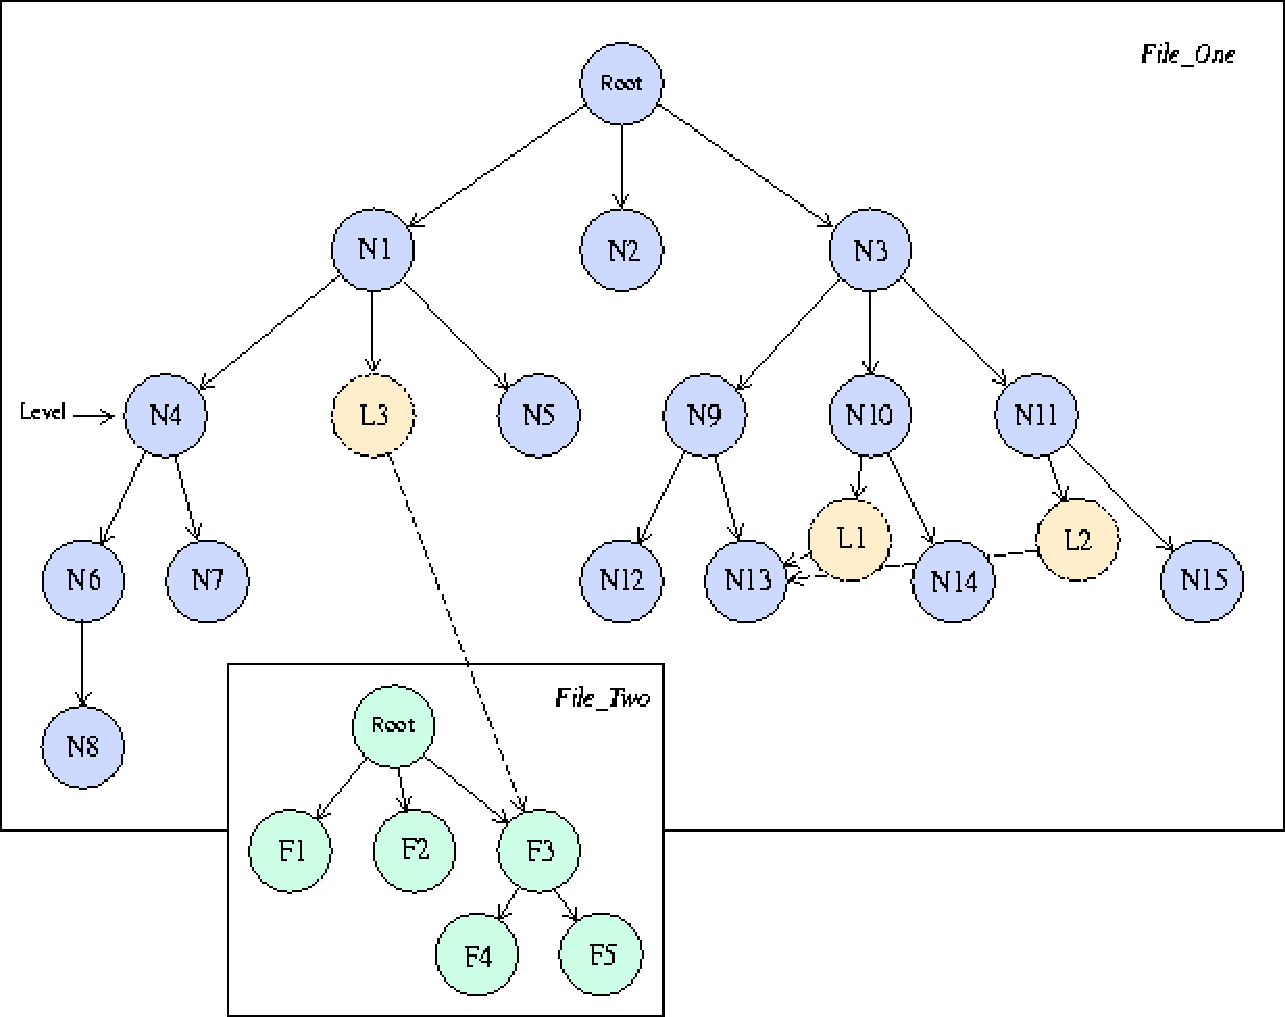
\includegraphics[width=6.0in]{figure}
   \caption{Example Database Hierarchy of Nodes}
   \label{f:example}
\end{figure}

A node knows about itself and its children, but it does not know
anything about its parent.
This means that it is possible to traverse ``down'' the tree by making
queries about what lies below the current node, but it is not possible
to traverse ``up'' the tree by making queries about nodes above a given
node.
If it is desired to move back up the tree, the user must keep track of
that information.

All database files start with a root node, which is created automatically
when a new file is opened.
There is only one root node in a database file, and may be referenced
by the database Root ID or by name as ``\key{/}''.

\subsection{Node Attributes}
\label{s:attributes}

Each node in the database may have zero to many subnodes that are
associated with it, as well as its own data.
The following are a list of attributes accessible by the user for a node
in the hierarchical database system.

\begin{Ventryi}{Number of Dimensions}
\item [Data]
      The data associated with a node.
\item [Data Type]
      A 2-byte character field, blank filled, case sensitive.
      Specifies the type of data (e.g., real, integer, character)
      associated with this node.
      The supported data types are listed in \autoref{t:datatype}
      on p.~\pageref*{t:datatype}.
\item [Dimensions]
      An integer vector containing the number of elements within
      each dimension.
      For example, if the array \fort{A} was declared (using Fortran) as
      \fort{A(10,20)}, the Dimension vector would contain two entries
      (10,20).
\item [ID]
      A unique identifier to access a given node within a file.
      This field contains sufficient information for the database manager
      to locate the node within a file.
      For any given node, the ID is generated only after the file it
      resides in has been opened by a program and the user requests
      information about the node.
      The ID is valid only within the program that opened the file and
      while that file is open.
      If the file is closed and reopened, the ID for any given node
      may be different.
      Within different programs, the node ID for the same node may
      also be different.
      The ID is never actually written into a file.
\item [Label]
      A 32-byte character field.
      The rules for Labels are identical to those for Names.
      Unlike names, Labels do not have to be unique.
      The Label field was introduced to allow ``data typing'' similar to
      the ``typedef'' concept in C.
      Using the Label field in this way allows programs to know some
      additional information about the use of the node itself or its
      child nodes and to call specific subroutines to read the data or
      react in specific ways upon detection of the type.
\item [Name]
      A 32-byte character field.
      The names of child nodes directly attached to a parent node must
      be unique.
      For example, in \autoref{f:example}, all nodes directly attached
      to N3 must have unique names.
      When a request to create a new node is made, the databse manager
      checks the requested name against the other names of the child
      nodes of the specified parent.
      If the requested name is not unique, an error is returned.

      Legal characteristics of a name are a A-Z, a-z, 0-9, and special
      characters (ASCII values from 32 to 126, except for the forward
      slash ``/'' (ASCII number 47)).
      Names will be blank filled to 32 bytes; they are case sensitive.
      Leading blanks are discarded and trailing blanks are ignored,
      whereas internal blanks are significant.

      \emph{Note}: Names passed from C must have the null
      ``\textbackslash0'' character appended to them.
      Names returned through the C interface will have the
      null character appended to them.
      Therefore, C programs should allocate 33 bytes for any Name in
      order to accommodate the null character.

      Fortran programs can allocate 32 characters for Names.
      The Fortran interface takes care of adding or removing the null
      character as required.
\item [Names of Subnodes]
      A list of names of the subnodes (children) of a node.
      (This is the information contained in the child table.)
\item [Number of Dimensions]
      The dimensionality of the data.
      ADF views all data as an array and can handle from zero (i.e., no
      data) to 12 dimensions.
      A ``0'' is used if the data type is empty.
      Thus, a scalar is viewed as a vector with one dimension and
      length 1.
\item [Number of Subnodes]
      The number of child nodes directly attached to any given node.
      Each node can have zero or more child nodes directly associated
      with it.
\item [Pointer]
      An address, from the point of view of a programming language.
      Pointers are like jumps, leading from one part of the data
      structure to another.
\end{Ventryi}

\subsection{Supported Data Types}

\begin{longtable}{l >{\quad}l >{\quad}l >{\quad}l}
\caption[Data Types]{\textbf{Data Types}}
\label{t:datatype}
\\ \hline\hline \\*[-2ex]
\bold{Notation} & \bold{Data Type} & \bold{C Type} & \bold{Fortran Type}
\\*[1ex] \hline\hline \\*[-2ex]
\key{MT} & No Data                 &  & \\
\key{I4} & 32-bit Integer          &  \key{int} & \fort{integer*4} \\
\key{I8} & 64-bit Integer          &  \key{cglong\_t} & \fort{integer*8}\\
\key{U4} & 32-bit Unsigned Integer &  \key{unsigned int} & \fort{integer*4} \\
\key{U8} & 64-bit Unsigned Integer &  \key{cgulong\_t} & \fort{integer*8} \\
\key{R4} & 32-bit Real             &  \key{float} & \fort{real*4} \\
\key{R8} & 64-bit Real             &  \key{double} & \fort{real*8} \\
\key{C1} & Character               &  \key{char} & \fort{character} \\
\key{B1} & Byte (unsigned byte)    &  \key{unsigned char} & \fort{character*1} \\
\key{LK} & Link                    &  &
\\*[1ex] \hline\hline
\end{longtable}

The \key{MT} node contains no data, and is typically used as a
container for subnodes (children).

A link is denoted by \key{LK}, and defines the
linkage between nodes and subnodes. A link provides a mechanism for
referring to a node that physically resides in a different part of the
hierarchy or a different database file. The link parallels a soft link
in the UNIX operating system in that it does not guarantee that the
referenced node exists. The database manager will ``resolve'' the link
only when information is requested about the linked node or it's children.

\subsection{Glossary of Terms}
\label{s:glossary}

\begin{Ventryi}{Node Name}
\item [Child]
      One of the subnodes of a Parent.
      A child node does not have knowledge of its parent node.
      The user must keep track of this relationship.
\item [Database]
      The representation of a hierarchy of nodes on disk files.
      By use of links, it may physically span multiple files.
\item [File]
      An database file, which a single root node and its underlying structure.
\item [ID]
      A unique identifier to access a given node within a database file.
      This field contains sufficient information for the database manager
      to locate the node within a file.
      For any given node, the ID is generated only after the file it
      resides in has been opened by a program and the user requests
      information about the node.
      The ID is valid only within the program that opened the file and
      while that file is open.
      If the file is closed and reopened, the ID for any given node
      may be different. Within different programs, the node-ID for the
      same node may also be different.
      The ID is never actually written into a file.
\item [Link-Node]
      A special type of node.
      Links are created using the
      \hyperlink{create_link}{\key{cgio\_create\_link}}
      subroutine.
      The data type of this node is \key{LK}, and its data is a
      one-dimensional array containing the name of the file (if other
      than the current file) containing the node to be linked and the
      full path name in that file from the root node to the desired
      node.

      Links provide a mechanism for referring to a node that physically
      resides in a different part of the hierarchy.
      The node pointed to by a link may or may not reside in the same
      file as the link itself.
      A link within ADF is very similar to a ``soft'' link in the
      UNIX operating system in that it does not guarantee that the
      referenced node exists.
      ADF will ``resolve'' the link only when information is requested
      about the node.
      If the ID of a link-node is used in an ADF call, the effect of
      the call is the same as if the ID of the linked-to node was used.
      Note that a link node does not have children itself.
      In \autoref{f:example} on p.~\pageref*{f:example}, the children
      seen for \key{L3} are \key{F4} and \key{F5}.
      If a child is ``added'' to \key{L3}, then in reality, the child
      is added to \key{F3}.
      There are specialized subroutines provided to create link nodes
      and extract the link details.
\item [Node]
      The single component used to construct a database.
\item [Node name]
      A node has a 32-character name.
      Every child node directly under a given parent must have a unique
      name.
      Legal characteristics in a name are \key{A-Z}, \key{a-z},
      \key{0-9}, and special characters (ASCII values from 32 to
      126, omitting the forward slash ``\key{/}'', ASCII number 47).
      Names will be blank filled to 32 bytes; they are case sensitive.
      Leading blanks are discarded and trailing blanks are ignored,
      whereas internal blanks are significant.
\item [Parent]
      A node that has subnodes directly associated with it.
\item [Pathname]
      Within a database, nodes can be referenced using the name of a node
      along with its parent ID, or by using a ``pathname'' whose syntax is
      roughly the same as a path name in the UNIX environment.
      A pathname that begins with a leading slash ``\key{/}'' is
      assumed to begin at the root node of the file.
      If no leading slash is given, the name is assumed to begin at the
      node specified by the parent ID.
      Although there is a 32-character limitation on the node Name,
      there is no restriction on the length of the pathname.
      For example, equivalent ways to refer to node \key{N8} in
      \autoref{f:example} are:
      \begin{itemize}
      \item Node-ID for \key{N6} and name = ``\key{N8}''
      \item Node-ID for \key{N4} and name = ``\key{N6/N8}''
      \item Node-ID for \key{N1} and name = ``\key{N4/N6/N8}''
      \item Node-ID for the \key{Root\_Node} and name =
            ``\key{/N1/N4/N6/N8}''
      \end{itemize}
\end{Ventryi}

\subsection{Conventions and Implementations}
\label{s:conventions}

\begin{Ventryi}{return codes}
\item [C]
      All input strings are to be null terminated.
      All returned strings will have the trailing blanks removed and
      will be null terminated.
      Variables declared to hold Names, Labels, and Data-Types should
      be at least 33 characters long.
      \textit{cgns\_io.h} has a number of variables defined.
      An example declaration would be:
\begin{indlefttt}
char name[CGIO\_MAX\_NAME\_LENGTH+1];
\end{indlefttt}
\item [Fortran]
      Strings will be determined using inherited length.
      Returned strings will be blank filled to the specified length.
      All returned names will be left justified and blank filled on the
      right.
      There will be no null character.
      An example declaration would be:
\begin{indlefttt}
PARAMETER CGIO\_MAX\_NAME\_LENGTH=32
CHARACTER*(CGIO\_MAX\_NAME\_LENGTH) NAME
\end{indlefttt}
      or include the Fortran header file \textit{cgns\_io\_f.h}
      which defines these parameters.
\item [ID]
      A unique identifier to access a given node within a database.
      For any given node, the ID is generated only after the file it
      resides in has been opened by a program and the user requests
      information about the node.
      The ID is valid only within the program that opened the file and
      while that file is open.
      If the file is closed and reopened, the ID for any given node
      may be different.
      Within different programs, the node ID for the same node may
      also be different.
      The ID is not ever actually written into a file.

      The declaration for variables that will hold node IDs should be
      for an 8-byte real number.
\item [Indexing]
      All indexing is Fortran-like in that the starting index is 1 and
      the last is \fort{N} for $N$ items in an index or array
      dimension.
      The array structure is assumed to be the same as in Fortran
      with the first array dimension varying the fastest and the last
      dimension varying the slowest.
 
      The index starting at one is used in
      \hyperlink{read_data}{\key{cgio\_read\_data}},
      \hyperlink{write_data}{\key{cgio\_write\_data}},
      \hyperlink{children_names}{\key{cgio\_children\_names}}, and
      \hyperlink{children_ids}{\key{cgio\_children\_ids}}.
 
      The user should be aware of the differences in array indexing
      between Fortran and C.
      The subroutines
      \hyperlink{read_all_data}{\key{cgio\_read\_all\_data}} and
      \hyperlink{write_all_data}{\key{cgio\_write\_all\_data}}
      merely take a pointer to the beginning of the data, compute how
      much data is to be read/written, and process as many bytes as
      have been requested.
      Thus, these routines effectively make a copy of memory onto disk
      or vice versa.
      Given this convention, it is possible for a C program to
      use standard C conventions for array indexing and use
      \key{cgio\_write\_all\_data} to store the array on disk.
      Then a Fortran program might use \key{cgio\_read\_all\_data} to
      read the data set.
      Unless the user is aware of the structure of the data, it is
      possible for the array to be transposed relative to what is
      expected.
 
      The implications of the assumed array structure convention can be
      quite subtle.
      The subroutines \key{cgio\_write\_data} and
      \key{cgio\_read\_data} assume the Fortran array structure in
      order to index the data.
      Again, unless the user is aware of the implications of this, it
      is possible to write an array on disk and later try to change a
      portion of the data and not change the correct numbers.
 
      As long as users are aware of how their data structure maps onto
      the database, there will not be any problems.
\item [return codes]
      The CGIO routines return an integer code indicating whether they
      were successfull or not. On success, 0 (\key{CGIO\_ERR\_NONE}) is
      returned. A non-zero return indicates an error. Return codes < 0
      indicate an error at the CGIO level; codes > 0 indicate an
      error in the database manager. See
      \hyperlink{s:messages}{Error Messages} for a list of
       error codes and mesages.
\end{Ventryi}

\subsection{Limits and Sizes}
\label{s:defaults}

The following default values, sizes, and limits are defined in the
header file \textit{cgns\_io.h}.

\begin{longtable}{l >{\quad}l >{\quad}l}
\caption[Default Values and Sizes]{\textbf{Default Values and Sizes}}
\label{t:defaults}
\\ \hline\hline \\*[-2ex]
\bold{Define} & \bold{Value} & \bold{Attribute}
\\*[1ex] \hline\hline \\*[-2ex]
\key{CGIO\_MAX\_DATATYPE\_LENGTH} & 2    & Data type length \\
\key{CGIO\_MAX\_DIMENSIONS}       & 12   & Maximum dimensions \\
\key{CGIO\_MAX\_NAME\_LENGTH}     & 32   & Name length \\
\key{CGIO\_MAX\_LABEL\_LENGTH}    & 32   & Label length \\
\key{CGIO\_MAX\_VERSION\_LENGTH}  & 32   & Version length \\
\key{CGIO\_MAX\_DATE\_LENGTH}     & 32   & Date length \\
\key{CGIO\_MAX\_ERROR\_LENGTH}    & 80   & Maximum length of error string \\
\key{CGIO\_MAX\_LINK\_DEPTH}      & 100  & Maximum link depth \\
\key{CGIO\_MAX\_FILE\_LENGTH}     & 1024 & File name length \\
\key{CGIO\_MAX\_LINK\_LENGTH}     & 4096 & Maximum link data size
\\*[1ex] \hline\hline\hline
\end{longtable}


\section{Database-Level Routines}
\label{s:database}

\begin{fctbox}
\textcolor{output}{\textit{ier}} = cgio\_is\_supported(\textcolor{input}{int file\_type}); & - - - \\
\textcolor{output}{\textit{ier}} = cgio\_check\_file(\textcolor{input}{const char *filename}, \textcolor{output}{\textit{int *file\_type}}); & - - - \\
\textcolor{output}{\textit{ier}} = cgio\_open\_file(\textcolor{input}{const char *filename}, \textcolor{input}{int file\_mode}, & r w m \\
~~~~~~~\textcolor{input}{int file\_type}, \textcolor{output}{\textit{int *cgio\_num}}); & \\
\textcolor{output}{\textit{ier}} = cgio\_close\_file(\textcolor{input}{int cgio\_num}); & r w m \\
\textcolor{output}{\textit{ier}} = cgio\_get\_file\_type(\textcolor{input}{int cgio\_num}, \textcolor{output}{\textit{int *file\_type}}); & r w m \\
\textcolor{output}{\textit{ier}} = cgio\_get\_root\_id(\textcolor{input}{int cgio\_num}, \textcolor{output}{\textit{double *rootid}}); & r w m \\
\hline
call cgio\_is\_supported\_f(\textcolor{input}{file\_type}, \textcolor{output}{\textit{ier}}) & - - - \\
call cgio\_check\_file\_f(\textcolor{input}{filename}, \textcolor{output}{\textit{file\_type}}, \textcolor{output}{\textit{ier}}) & - - - \\
call cgio\_open\_file\_f(\textcolor{input}{filename}, \textcolor{input}{file\_mode}, \textcolor{input}{file\_type}, \textcolor{output}{\textit{cgio\_num}}, \textcolor{output}{\textit{ier}}) & r w m \\
call cgio\_close\_file\_f(\textcolor{input}{cgio\_num}, \textcolor{output}{\textit{ier}}) & r w m \\
call cgio\_get\_file\_type\_f(\textcolor{input}{cgio\_num}, \textcolor{output}{\textit{file\_type}}, \textcolor{output}{\textit{ier}}) & r w m \\
call cgio\_get\_root\_id\_f(\textcolor{input}{cgio\_num}, \textcolor{output}{\textit{rootid}}, \textcolor{output}{\textit{ier}}) & r w m \\
\end{fctbox}

\noindent
\textbf{\textcolor{input}{Input}/\textcolor{output}{\textit{Output}}}

\begin{Ventryi}{\texttt{file\_type}}\raggedright
\item [\texttt{file\_type}]
      Type of database file. acceptable values are \texttt{CGIO\_FILE\_NONE},
      \texttt{CGIO\_FILE\_ADF}, \texttt{CGIO\_FILE\_HDF5} and
      \texttt{CGIO\_FILE\_ADF2}.
\item [\texttt{filename}]
      Name of the database file, including path name if necessary.
      There is no limit on the length of this character variable.
\item [\texttt{file\_mode}]
      Mode used for opening the file.
      The supported modes are \texttt{CGIO\_MODE\_READ},
      \texttt{CGIO\_MODE\_WRITE}, and \texttt{CGIO\_MODE\_MODIFY}.
\item [\texttt{cgio\_num}]
      Indentifier for the open database file.
\item [\texttt{rootid}]
      Ndeo identifier for the root node of the database.
\item [\texttt{ier}]
      Error status.
\end{Ventryi}

\subsection{Function Descriptions}

\subsubsection{\texttt{cgio\_is\_supported}} \label{is_supported}
    \noindent
    Determines if the database type given by \texttt{file\_type} is supported
    by the library. Retuns 0 if supported, else \texttt{CGIO\_ERR\_FILE\_TYPE}
    if not. \texttt{CGIO\_FILE\_ADF} is always supported;
    \texttt{CGIO\_FILE\_HDF5} is supported if the library was built with HDF5;
    and \texttt{CGIO\_FILE\_ADF2} is supported when built in 32-bit mode.

\subsubsection{\texttt{cgio\_check\_file}} \label{check_file}
    \noindent
    Checks the file \texttt{filename} to determine if it is a valid database.
    If so, returns 0 and the type of database in \texttt{file\_type},
    otherwise returns an error code and \texttt{file\_type} will be set
    to \texttt{CGIO\_FILE\_NONE}.

\subsubsection{\texttt{cgio\_open\_file}} \label{open_file}
    \noindent
    Opens a database file of the specified type and mode. If successfull,
    returns 0, and the database identifier in \texttt{cgio\_num}, otherwise
    returns an error code. The database identifier is used to access the
    database in subsequent function calls.

    \noindent
    The mode in which the database is opened is given by \texttt{file\_mode},
    which may take the value \texttt{CGIO\_MODE\_READ}, \texttt{CGIO\_MODE\_WRITE},
    or \texttt{CGIO\_MODE\_MODIFY}. New databases should be opened with
    \texttt{CGIO\_MODE\_WRITE}, while existing databases are opened with either
    \texttt{CGIO\_MODE\_READ} (for read-only access) or
    \texttt{CGIO\_MODE\_MODIFY} (for read/write access).
 
    \noindent
    A specific database type may be specified by \texttt{file\_type}, which may
    be one of \texttt{CGIO\_FILE\_NONE}, \texttt{CGIO\_FILE\_ADF},
    \texttt{CGIO\_FILE\_HDF5}, or \texttt{CGIO\_FILE\_ADF2}. When opening a database
    in write mode, \texttt{CGIO\_FILE\_NONE} indicates that the default database
    type should be used, otherwise the specified database type will be opened.
    When opening in read or modify mode, \texttt{CGIO\_FILE\_NONE} indicates that
    any database type is acceptable, otherwise if the database type does
    not match that given by \texttt{file\_type} an error will be retuned.

\subsubsection{\texttt{cgio\_close\_file}} \label{close_file}
    \noindent
    Closes the database given by \texttt{cgio\_num}. Returns 0 for success,
    else an error code.

\subsubsection{\texttt{cgio\_get\_file\_type}} \label{get_file_type}
    \noindent
    Gets the type of the database given by \texttt{cgio\_num}.
    Returns 0 and the type in \texttt{file\_type} if successfull,
    else an error code.

\subsubsection{\texttt{cgio\_get\_root\_id}} \label{get_root_id}
    \noindent
    Gets the unique node identifier for the root node in the database given
    by \texttt{cgio\_num}. Returns 0 and the identifier in \texttt{rootid}
    if successfull, else an error code.



\section{Data Structure Management Routines}
\label{s:structure}

\begin{fctbox}
\textcolor{output}{\textit{ier}} = cgio\_create\_node(\textcolor{input}{int cgio\_num}, \textcolor{input}{double pid}, \textcolor{input}{const char *name}, & - w m \\
~~~~~~~\textcolor{output}{\textit{double *id}}); & \\
\textcolor{output}{\textit{ier}} = cgio\_new\_node(\textcolor{input}{int cgio\_num}, \textcolor{input}{double pid}, \textcolor{input}{const char *name}, & - w m \\
~~~~~~~\textcolor{input}{const char *label}, \textcolor{input}{const char *data\_type}, \textcolor{input}{int ndims}, & \\
~~~~~~~\textcolor{input}{const cgsize\_tt *dims}, \textcolor{input}{const void *data}, \textcolor{output}{\textit{double *id}}); & \\
\textcolor{output}{\textit{ier}} = cgio\_delete\_node(\textcolor{input}{int cgio\_num}, \textcolor{input}{double pid}, \textcolor{input}{double id}); & - w m \\
\textcolor{output}{\textit{ier}} = cgio\_move\_node(\textcolor{input}{int cgio\_num}, \textcolor{input}{double pid}, \textcolor{input}{double id}, & - w m \\
~~~~~~~\textcolor{input}{double new\_pid}); & \\
\textcolor{output}{\textit{ier}} = cgio\_number\_children(\textcolor{input}{int cgio\_num}, \textcolor{input}{double id}, \textcolor{output}{\textit{int *num\_child}}); & r w m \\
\textcolor{output}{\textit{ier}} = cgio\_children\_names(\textcolor{input}{int cgio\_num}, \textcolor{input}{double id}, \textcolor{input}{int start}, & r w m \\
~~~~~~~\textcolor{input}{int max\_ret}, \textcolor{input}{int name\_len}, \textcolor{output}{\textit{int *num\_ret}}, \textcolor{output}{\textit{char *child\_names}}); & \\
\textcolor{output}{\textit{ier}} = cgio\_children\_ids(\textcolor{input}{int cgio\_num}, \textcolor{input}{double id}, \textcolor{input}{int start}, & r w m \\
~~~~~~~\textcolor{input}{int max\_ret}, \textcolor{output}{\textit{int *num\_ret}}, \textcolor{output}{\textit{char *child\_ids}}); & \\
\hline
call cgio\_create\_node\_f(\textcolor{input}{cgio\_num}, \textcolor{input}{pid}, \textcolor{input}{name}, \textcolor{output}{\textit{id}}, \textcolor{output}{\textit{ier}}) & - w m \\
call cgio\_new\_node\_f(\textcolor{input}{cgio\_num}, \textcolor{input}{pid}, \textcolor{input}{name}, \textcolor{input}{label}, \textcolor{input}{data\_type}, \textcolor{input}{ndims}, & - w m \\
~~~~~\textcolor{input}{dims}, \textcolor{input}{data}, \textcolor{output}{\textit{id}}, \textcolor{output}{\textit{ier}}); & \\
call cgio\_delete\_node\_f(\textcolor{input}{cgio\_num}, \textcolor{input}{pid}, \textcolor{input}{id}, \textcolor{output}{\textit{ier}}) & - w m \\
call cgio\_move\_node\_f(\textcolor{input}{cgio\_num}, \textcolor{input}{pid}, \textcolor{input}{id}, \textcolor{input}{new\_pid}, \textcolor{output}{\textit{ier}}) & - w m \\
call cgio\_number\_children\_f(\textcolor{input}{cgio\_num}, \textcolor{input}{id}, \textcolor{output}{\textit{num\_child}}, \textcolor{output}{\textit{ier}}) & r w m \\
call cgio\_children\_names\_f(\textcolor{input}{cgio\_num}, \textcolor{input}{id}, \textcolor{input}{start}, \textcolor{input}{max\_ret}, \textcolor{input}{name\_len}, & r w m \\
~~~~~\textcolor{output}{\textit{num\_ret}}, \textcolor{output}{\textit{child\_names}}, \textcolor{output}{\textit{ier}}) & \\
call cgio\_children\_ids\_f(\textcolor{input}{cgio\_num}, \textcolor{input}{id}, \textcolor{input}{start}, \textcolor{input}{max\_ret}, & r w m \\
~~~~~\textcolor{output}{\textit{num\_ret}}, \textcolor{output}{\textit{child\_ids}}, \textcolor{output}{\textit{ier}}) & \\
\end{fctbox}

\noindent
\textbf{\textcolor{input}{Input}/\textcolor{output}{\textit{Output}}}

\begin{Ventryi}{\texttt{child\_names}}\raggedright
\item [\texttt{cgio\_num}]
      Database identifier.
\item [\texttt{pid}]
      Parent node identifier.
\item [\texttt{id}]
      Node identifier.
\item [\texttt{name}]
      Node name (max length 32).
\item [\texttt{label}]
      Node label (max length 32).
\item [\texttt{data\_type}]
      Type of data contained in the node. One of ``MT'', ``I4'', ``I8'',
      ``U4'', ``U8'', ``R4'', ``C1'', or ``B1''.
\item [\texttt{ndims}]
      Number of dimensions for the data (max 12).
\item [\texttt{dims}]
      Data dimension values (\texttt{ndims} values).
\item [\texttt{data}]
      Data array to be stored with the node.
\item [\texttt{new\_pid}]
      New parent node identifier under which the node is to be moved.
\item [\texttt{num\_child}]
      Number of children of the specified node.
\item [\texttt{start}]
      Starting index for returned child names or ids
      (1 <= \texttt{start} <= \texttt{num\_child}).
\item [\texttt{max\_ret}]
      Maximum child names or ids to be returned
      (1 <= \texttt{max\_ret} <= \texttt{num\_child-start+1}).
\item [\texttt{name\_len}]
      Length reserved for each returned child name.
\item [\texttt{num\_ret}]
      Number of returned values of child names or identifiers.
\item [\texttt{child\_names}]
      Child node names (\texttt{num\_ret} values). This array should
      be dimensioned at least (\texttt{name\_len * max\_ret}).
\item [\texttt{child\_ids}]
      Child node identifiers (\texttt{num\_ret} values). This array
       should be dimensioned at least (\texttt{max\_ret}).
\item [\texttt{ier}]
      Error status.
\end{Ventryi}

\subsection{Function Descriptions}

\subsubsection{\texttt{cgio\_create\_node}} \label{create_node}
    \noindent
    Creates a new empty node in the database given by \texttt{cgio\_num}
    as a child of the node identified by \texttt{pid}. The name of the new
    node is given by \texttt{name}, and must not already exist as a child
    of the parent node. The node will contain no label, dimensions,
    or data. Use the \hyperlink{s:node}{Node Management Routines} to
    change the properties of the node, and the
    \hyperlink{s:dataio}{Data I/O Routines} to add data. Returns 0 and the
    identifier of the new node in \texttt{id} on success, else an error code.

\subsubsection{\texttt{cgio\_new\_node}} \label{new_node}
    \noindent
    Creates a new node in the database given by \texttt{cgio\_num}
    as a child of the node identified by \texttt{pid}. The name of the new
    node is given by \texttt{name}, and must not already exist as a child
    of the parent node. The node label is given by \texttt{label},
    the type of data by \texttt{data\_type}, the dimensions of the data by
    \texttt{ndims} and \texttt{dims}, and the data to write to the node
    by \texttt{data}. This is equivalent to calling the routines:
    \hyperlink{create_node}{\texttt{cgio\_create\_node}},
    \hyperlink{set_label}{\texttt{cgio\_set\_label}}.
    \hyperlink{set_dimensions}{\texttt{cgio\_set\_dimensions}}, and
    \hyperlink{write_all_data}{\texttt{cgio\_write\_all\_data}}
    Returns 0 and the identifier of the new node in \texttt{id} on success,
    else an error code.

\subsubsection{\texttt{cgio\_delete\_node}} \label{delete_node}
    \noindent
    Deletes the node identified by \texttt{id} below the parent node identified
    by \texttt{pid} in the database given by \texttt{cgio\_num}. All children
    of the deleted node will also be deleted unless a link is encountered.
    The link node will be deleted but nothing below it.
    Returns 0 on success, else an error code.

\subsubsection{\texttt{cgio\_move\_node}} \label{move_node}
    \noindent
    Moves the node indentified by \texttt{id} below the parent node identified
    by \texttt{pid} to below the new parent node identified by \texttt{new\_pid}
    in the database given by \texttt{cgio\_num}. A node by the same name as
    that that for \texttt{id} must not already exist under \texttt{new\_pid}.
    A node may only be moved if it and the parent nodes all reside in the
    sane physical database. Returns 0 on success, else an error code.

\subsubsection{\texttt{cgio\_number\_children}} \label{number_children}
    \noindent
    Gets the number of children of the node identified by \texttt{id} in the
    database given by \texttt{cgio\_num}, Returns 0 and the number of children
    in \texttt{num\_child} on success, else an error code.

\subsubsection{\texttt{cgio\_children\_names}} \label{children_names}
    \noindent
    Gets the names of the children of the node identified by \texttt{id} in
    the database given by \texttt{cgio\_num}. The starting index for the
    array of names is given by \texttt{start}, and the maximum number of
    names to return by \texttt{max\_ret}. Both \texttt{start} and \texttt{max\_ret}
    should be between 1 and \texttt{num\_child}, inclusively. The size reserved
    for each name in \texttt{child\_names} is given by \texttt{name\_len}.
    The array \texttt{child\_names} should be dimensioned at least
    (\texttt{name\_len * max\_ret}). Since node names are limited to a length
    of \texttt{CGIO\_MAX\_NAME\_LENGHT} (32), \texttt{name\_len} should be at
    least 32 to ensure the returned names are mot truncated. In C, an
    additional byte should be added to \texttt{name\_len} allow for the
    terminating '0' for each name. If successfull, the function returns 0;
    the actual number of returned names is given by \texttt{num\_ret},
    and the array of names in \texttt{child\_names}. In C, the names are
    '0'-terminated within each name field. In Fortran, any unused space
    is padded with blanks (space character).

\subsubsection{\texttt{cgio\_children\_ids}} \label{children_ids}
    \noindent
    Gets the node identifiers of the children of the node identified by
    \texttt{id} in the database given by \texttt{cgio\_num}.
    The starting index for the array of ids is given by \texttt{start},
    and the maximum ids to return by \texttt{max\_ret}. Both \texttt{start}
    and \texttt{max\_ret} should be between 1 and \texttt{num\_child}, inclusively.
    The array \texttt{child\_ids} should be dimensioned at least
    (\texttt{max\_ret}). If successfull, the function returns 0; the
    actual number of returned ids is given by \texttt{num\_ret}, and the
    array of identifiers in \texttt{child\_ids}.


\section{Links}
\label{s:links}
\thispagestyle{plain}

\begin{fctbox}
\textcolor{output}{\textit{ier}} = cg\_link\_write(\textcolor{input}{char *nodename}, \textcolor{input}{char *filename}, & - w m \\
~~~~~~\textcolor{input}{char *name\_in\_file}); & \\
\textcolor{output}{\textit{ier}} = cg\_is\_link(\textcolor{output}{\textit{int *path\_length}}); & r - m \\
\textcolor{output}{\textit{ier}} = cg\_link\_read(\textcolor{output}{\textit{char **filename}}, \textcolor{output}{\textit{char **link\_path}}); & r - m \\
\hline
call cg\_link\_write\_f(\textcolor{input}{nodename}, \textcolor{input}{filename}, \textcolor{input}{name\_in\_file}, \textcolor{output}{\textit{ier}}) & - w m \\
call cg\_is\_link\_f(\textcolor{output}{\textit{path\_length}}, \textcolor{output}{\textit{ier}}) & r - m \\
call cg\_link\_read\_f(\textcolor{output}{\textit{filename}}, \textcolor{output}{\textit{link\_path}}, \textcolor{output}{\textit{ier}}) & r - m \\
\end{fctbox}

\noindent
\textbf{\textcolor{input}{Input}/\textcolor{output}{\textit{Output}}}

\begin{Ventryi}{\fort{name\_in\_file}}\raggedright
\item [\fort{nodename}]
      Name of the link node to create, e.g., \fort{GridCoordinates}.
      (\textcolor{input}{Input})
\item [\fort{filename}]
      Name of the linked file, or empty string if the link is within the
      same file.
      (\textcolor{input}{Input} for \fort{cg\_link\_write};
      \textcolor{output}{\textit{output}} for \fort{cg\_link\_read})
\item [\fort{name\_in\_file}]
      Path name of the node which the link points to.
      This can be a simple or a compound name, e.g.,
      \fort{Base/Zone 1/GridCoordinates}.
      (\textcolor{input}{Input})
\item [\fort{path\_length}]
      Length of the path name of the linked node.
      The value 0 is returned if the node is not a link.
      (\textcolor{output}{\textit{Output}})
\item [\fort{link\_path}]
      Path name of the node which the link points to.
      (\textcolor{output}{\textit{Output}})
\item [\fort{ier}]
      Error status.
      (\textcolor{output}{\textit{Output}})
\end{Ventryi}

Use \fort{cg\_goto(\_f)}, described in \autoref{s:navigating}, to
position to a location in the file prior to calling these routines.

When using \fort{cg\_link\_write}, the node being linked to does not have 
to exist when the link is created.
However, when the link is used, an error will occur if the linked-to
node does not exist.

Only nodes that support child nodes will support links.

It is assumed that the CGNS version for the file containing the link,
as determined by the \fort{CGNSLibraryVersion\_t} node, is also
applicable to \fort{filename}, the file containing the linked node.

Memory is allocated by the library for the return values of the C
function \fort{cg\_link\_read}.
This memory should be freed by the user when no longer needed by calling
\texttt{cg\_free(filename)} and \texttt{cg\_free(link\_path)}, described
in \autoref{s:free}.

\section{Node Management Routines}
\label{s:node}

\begin{fctbox}
\textcolor{output}{\textit{ier}} = cgio\_get\_node\_id(\textcolor{input}{int cgio\_num}, \textcolor{input}{double pid}, \textcolor{input}{const char *pathname}, & r w m \\
~~~~~~~\textcolor{output}{\textit{double *id}}); & \\
\textcolor{output}{\textit{ier}} = cgio\_get\_name(\textcolor{input}{int cgio\_num}, \textcolor{input}{double id}, \textcolor{output}{\textit{char *name}}); & r w m \\
\textcolor{output}{\textit{ier}} = cgio\_set\_name(\textcolor{input}{int cgio\_num}, \textcolor{input}{double pid}, \textcolor{input}{double id}, & - w m \\
~~~~~~~\textcolor{input}{const char *name}); & \\
\textcolor{output}{\textit{ier}} = cgio\_get\_label(\textcolor{input}{int cgio\_num}, \textcolor{input}{double id}, \textcolor{output}{\textit{char *label}}); & r w m \\
\textcolor{output}{\textit{ier}} = cgio\_set\_label(\textcolor{input}{int cgio\_num}, \textcolor{input}{double id}, \textcolor{input}{const char *label}); & - w m \\
\textcolor{output}{\textit{ier}} = cgio\_get\_data\_type(\textcolor{input}{int cgio\_num}, \textcolor{input}{double id}, \textcolor{output}{\textit{char *data\_type}}); & r w m \\
\textcolor{output}{\textit{ier}} = cgio\_get\_dimensions(\textcolor{input}{int cgio\_num}, \textcolor{input}{double id}, \textcolor{output}{\textit{int *ndims}}, & r w m \\
~~~~~~~\textcolor{output}{\textit{cgsize\_t *dims}}); & \\
\textcolor{output}{\textit{ier}} = cgio\_set\_dimensions(\textcolor{input}{int cgio\_num}, \textcolor{input}{double id}, & - w m \\
~~~~~~~\textcolor{input}{const char *data\_type}, \textcolor{input}{int ndims}, \textcolor{input}{const cgsize\_t *dims}); & \\
\hline
call cgio\_get\_node\_id\_f(\textcolor{input}{cgio\_num}, \textcolor{input}{pid}, \textcolor{input}{name}, \textcolor{output}{\textit{id}}, \textcolor{output}{\textit{ier}}) & r w m \\
call cgio\_get\_name\_f(\textcolor{input}{cgio\_num}, \textcolor{input}{id}, \textcolor{output}{\textit{name}}, \textcolor{output}{\textit{ier}}) & r w m \\
call cgio\_set\_name\_f(\textcolor{input}{cgio\_num}, \textcolor{input}{pid}, \textcolor{input}{id}, \textcolor{input}{name}, \textcolor{output}{\textit{ier}}) & - w m \\
call cgio\_get\_label\_f(\textcolor{input}{cgio\_num}, \textcolor{input}{id}, \textcolor{output}{\textit{label}}, \textcolor{output}{\textit{ier}}) & r w m \\
call cgio\_set\_label\_f(\textcolor{input}{cgio\_num}, \textcolor{input}{id}, \textcolor{input}{label}, \textcolor{output}{\textit{ier}}) & - w m \\
call cgio\_get\_data\_type\_f(\textcolor{input}{cgio\_num}, \textcolor{input}{id}, \textcolor{output}{\textit{data\_type}}, \textcolor{output}{\textit{ier}}) & r w m \\
call cgio\_get\_dimensions\_f(\textcolor{input}{cgio\_num}, \textcolor{input}{id}, \textcolor{output}{\textit{ndims}}, \textcolor{output}{\textit{dims}}, \textcolor{output}{\textit{ier}}) & r w m \\
call cgio\_set\_dimensions\_f(\textcolor{input}{cgio\_num}, \textcolor{input}{id}, \textcolor{input}{data\_type}, \textcolor{input}{ndims}, \textcolor{input}{dims}, \textcolor{output}{\textit{ier}}) & - w m \\
\end{fctbox}

\noindent
\textbf{\textcolor{input}{Input}/\textcolor{output}{\textit{Output}}}

\begin{Ventryi}{\texttt{data\_type}}\raggedright
\item [\texttt{cgio\_num}]
      Database identifier.
\item [\texttt{pid}]
      Parent node identifier.
\item [\texttt{id}]
      Node identifier.
\item [\texttt{pathname}]
      Absolute or relative path name for a node.
\item [\texttt{name}]
      Node name (max length 32).
\item [\texttt{label}]
      Node label (max length 32).
\item [\texttt{data\_type}]
      Type of data contained in the node. One of ``MT'', ``I4'', ``I8'',
      ``U4'', ``U8'', ``R4'', ``C1'', or ``B1''.
\item [\texttt{ndims}]
      Number of dimensions for the data (max 12).
\item [\texttt{dims}]
      Data dimension values (\texttt{ndims} values).
\item [\texttt{ier}]
      Error status.
\end{Ventryi}

\subsection{Function Descriptions}

\subsubsection{\texttt{cgio\_get\_node\_id}} \label{get_node_id}
    \noindent
    Gets the node identifier for the node specified by \texttt{pathname}
    in the database given by \texttt{cgio\_num}. if \texttt{pathname} starts
    with ``\texttt{/}'', then it is taken as an absolute path and is located based
    on the root id of the database, otherwise it is taken to be a relative
    path from the parent node identifed by \texttt{pid}. The function returns
    0 and the node identifier in \texttt{id} on success, else an error code.

\subsubsection{\texttt{cgio\_get\_name}} \label{get_name}
    \noindent
    Gets the name of the node identified by \texttt{id} in the database given
    by \texttt{cgio\_num}. The name is returned in \texttt{name}, and has a
    maximum length of \texttt{CGIO\_MAX\_NAME\_LENGTH} (32). In C, \texttt{name}
    should be dimensioned at least 33 to allow for the terminating '0'.
    The function returns 0 for success, else an error code.

\subsubsection{\texttt{cgio\_set\_name}} \label{set_name}
    \noindent
    Sets (renames) the node identied by \texttt{id} in the database given by
    \texttt{cgio\_num} to \texttt{name}. The parent node identifier is given
    by \texttt{pid}. There must not already exist a child node of \texttt{pid}
    with that name. The function return 0 on success, else an error code.

\subsubsection{\texttt{cgio\_get\_label}} \label{get_label}
    \noindent
    Gets the label of the node identified by \texttt{id} in the database given
    by \texttt{cgio\_num}. The label is returned in \texttt{label}, and has a
    maximum length of \texttt{CGIO\_MAX\_LABEL\_LENGTH} (32). In C, \texttt{label}
    should be dimensioned at least 33 to allow for the terminating '0'.
    The function returns 0 for success, else an error code.

\subsubsection{\texttt{cgio\_set\_label}} \label{set_label}
    \noindent
    Sets the label of the node identied by \texttt{id} in the database given by
    \texttt{cgio\_num} to \texttt{label}. The function return 0 on success,
    else an error code.

\subsubsection{\texttt{cgio\_get\_data\_type}} \label{get_data_type}
    \noindent
    Gets the data type of the data associated with the node identified by
    \texttt{id} in the database given by \texttt{cgio\_num}.
    The data type is returned in \texttt{data\_type}, and has a
    maximum length of \texttt{CGIO\_MAX\_DATATYPE\_LENGTH} (2).
    In C, \texttt{data\_type} should be dimensioned at least 3 to allow for
    the terminating '0'.
    The function returns 0 for success, else an error code.

\subsubsection{\texttt{cgio\_get\_dimensions}} \label{get_dimensions}
    \noindent
    Gets the dimensions of the data associated with the node identified by
    \texttt{id} in the database given by \texttt{cgio\_num}. The number of
    dimensions is returned in \texttt{ndims} and the dimension values
    in \texttt{dims}. Since the maximum number of dimensions is
    \texttt{CGIO\_MAX\_DIMENSIONS} (12), \texttt{dims} should be dimensioned
    12, unless the actual number of dimensions is already known.
    The function returns 0 for success, else an error code.

\subsubsection{\texttt{cgio\_set\_dimensions}} \label{set_dimensions}
    \noindent
    Sets the data type and dimensions for data associated with the node
    identified by \texttt{id} in the database given by \texttt{cgio\_num}.
    The data type (\texttt{data\_type}) as one of:
    \begin{Ventryi}{``\texttt{MT}''}
    \item [``\texttt{MT}'']
          An empty node containing no data
    \item [``\texttt{I4}'']
          32-bit integer (int or integer*4)
    \item [``\texttt{I8}'']
          64-bit integer (cglong\_t or integer*8)
    \item [``\texttt{U4}'']
          32-bit unsigned integer (unsigned int or integer*4)
    \item [``\texttt{U8}'']
          64-bit unsigned integer (cgulong\_t or integer*8)
    \item [``\texttt{R4}'']
          32-bit real (float or real*4)
    \item [``\texttt{R8}'']
          64-bit real (double or real*8)
    \item [``\texttt{C1}'']
          character (char or character)
    \item [``\texttt{B1}'']
          unsigned bytes (unsigned char or character*1)
    \end{Ventryi}
    \noindent
    The number of dimensions is given by \texttt{ndims} (maximum is 12), and
    the dimension values by \texttt{dims}. Note that any existing data for the
    node will be destroyed. To add the data to the node, use one of the
    \hyperlink{s:dataio}{data writing routines}. The function returns 0 for
    success, else an error code.


\section{Data I/O Routines}
\label{s:dataio}

\begin{fctbox}
\textcolor{output}{\textit{ier}} = cgio\_read\_data(\textcolor{input}{int cgio\_num}, \textcolor{input}{double id}, \textcolor{input}{const cgsize\_t *s\_start}, & r w m \\
~~~~~~~\textcolor{input}{const cgsize\_t *s\_end}, \textcolor{input}{const cgsize\_t *s\_stride}, \textcolor{input}{int m\_num\_dims}, & \\
~~~~~~~\textcolor{input}{const cgsize\_t *m\_dims}, \textcolor{input}{const cgsize\_t *m\_start}, & \\
~~~~~~~\textcolor{input}{const cgsize\_t *m\_end}, \textcolor{input}{const cgsize\_t *m\_stride}, \textcolor{output}{\textit{void *data}}); & \\
\textcolor{output}{\textit{ier}} = cgio\_read\_all\_data(\textcolor{input}{int cgio\_num}, \textcolor{input}{double id}, \textcolor{output}{\textit{void *data}}); & r w m \\
\textcolor{output}{\textit{ier}} = cgio\_read\_block\_data(\textcolor{input}{int cgio\_num}, \textcolor{input}{double id}, \textcolor{input}{cgsize\_t b\_start}, & r w m \\
~~~~~~~\textcolor{input}{cgsize\_t b\_end}, \textcolor{output}{\textit{void *data}}); & \\
\textcolor{output}{\textit{ier}} = cgio\_write\_data(\textcolor{input}{int cgio\_num}, \textcolor{input}{double id}, \textcolor{input}{const cgsize\_t *s\_start}, & - w m \\
~~~~~~~\textcolor{input}{const cgsize\_t *s\_end}, \textcolor{input}{const cgsize\_t *s\_stride}, \textcolor{input}{int m\_num\_dims}, & \\
~~~~~~~\textcolor{input}{const cgsize\_t *m\_dims}, \textcolor{input}{const cgsize\_t *m\_start}, & \\
~~~~~~~\textcolor{input}{const cgsize\_t *m\_end}, \textcolor{input}{const cgsize\_t *m\_stride}, \textcolor{input}{void *data}); & \\
\textcolor{output}{\textit{ier}} = cgio\_write\_all\_data(\textcolor{input}{int cgio\_num}, \textcolor{input}{double id}, \textcolor{input}{void *data}); & - w m \\
\textcolor{output}{\textit{ier}} = cgio\_write\_block\_data(\textcolor{input}{int cgio\_num}, \textcolor{input}{double id}, \textcolor{input}{cgsize\_t b\_start}, & - w m \\
~~~~~~~\textcolor{input}{cgsize\_t b\_end}, \textcolor{input}{void *data}); & \\
\hline
call cgio\_read\_data\_f(\textcolor{input}{cgio\_num}, \textcolor{input}{id}, \textcolor{input}{s\_start}, \textcolor{input}{s\_end}, \textcolor{input}{s\_stride},  & r w m \\
~~~~~~\textcolor{input}{m\_num\_dims}, \textcolor{input}{m\_dims}, \textcolor{input}{m\_start}, \textcolor{input}{m\_end}, \textcolor{input}{m\_stride}, \textcolor{output}{\textit{data}}, \textcolor{output}{\textit{ier}}) & \\
call cgio\_read\_all\_data\_f(\textcolor{input}{cgio\_num}, \textcolor{input}{id}, \textcolor{output}{\textit{data}}, \textcolor{output}{\textit{ier}}) & r w m \\
call cgio\_read\_block\_data\_f(\textcolor{input}{cgio\_num}, \textcolor{input}{id}, \textcolor{input}{b\_start}, \textcolor{input}{b\_end}, \textcolor{output}{\textit{data}}, \textcolor{output}{\textit{ier}}) & r w m \\
call cgio\_write\_data\_f(\textcolor{input}{cgio\_num}, \textcolor{input}{id}, \textcolor{input}{s\_start}, \textcolor{input}{s\_end}, \textcolor{input}{s\_stride}, & - w m \\
~~~~~~\textcolor{input}{m\_num\_dims}, \textcolor{input}{m\_dims}, \textcolor{input}{m\_start}, \textcolor{input}{m\_end}, \textcolor{input}{m\_stride}, \textcolor{input}{data}, \textcolor{output}{\textit{ier}}) & \\
call cgio\_write\_all\_data\_f(\textcolor{input}{cgio\_num}, \textcolor{input}{id}, \textcolor{input}{data}, \textcolor{output}{\textit{ier}}) & - w m \\
call cgio\_write\_block\_data\_f(\textcolor{input}{cgio\_num}, \textcolor{input}{id}, \textcolor{input}{b\_start}, \textcolor{input}{b\_end}, \textcolor{input}{data}, \textcolor{output}{\textit{ier}}) & - w m \\
\end{fctbox}

\noindent
\textbf{\textcolor{input}{Input}/\textcolor{output}{\textit{Output}}}

\begin{Ventryi}{\texttt{m\_num\_dims}}\raggedright
\item [\texttt{cgio\_num}]
      Database identifier.
\item [\texttt{id}]
      Node identifier.
\item [\texttt{s\_start}]
      Starting indices for data in the database.
      Fortran indexing is used (starting at 1).
\item [\texttt{s\_end}]
      Ending indices for data in the database.
      Fortran indexing is used (starting at 1).
\item [\texttt{s\_stride}]
      Step increment for data in the database.
\item [\texttt{m\_num\_dims}]
      Number of dimensions for data in memory.
\item [\texttt{m\_dims}]
      Dimension values for data in memory.
\item [\texttt{m\_start}]
      Starting indices for data in memory.
      Fortran indexing is used (starting at 1).
\item [\texttt{m\_end}]
      Ending indices for data in memory.
      Fortran indexing is used (starting at 1).
\item [\texttt{m\_stride}]
      Step increment for data in memory.
\item [\texttt{data}]
      Array of data to be read or written.
\item [\texttt{b\_start}]
      Starting offset (index) for the data in the database.
      Fortran indexing is used (starting at 1).
\item [\texttt{b\_end}]
      Ending offset (index) for the data in the database.
      Fortran indexing is used (starting at 1).
\item [\texttt{ier}]
      Error status.
\end{Ventryi}

\subsection{Function Descriptions}

\subsubsection{\texttt{cgio\_read\_data}} \label{read_data}
    \noindent
    This routine provides general purpose read capabilities from the
    node identified by \texttt{id} in the database given by \texttt{cgio\_num}.
    It allows for a general specification of the starting location within
    the data as well as fixed step lengths (strides) through the data from
    the initial position.
    This capability works for both the data on disk and the data being
    stored in memory. One set of vectors (\texttt{s\_start},
    \texttt{s\_end} and \texttt{s\_stride}) are used to describe the mapping
    of the data within the node, and a second set of vectors
    (\texttt{m\_start}, \texttt{m\_end} and \texttt{m\_stride}) are used to
    describe the mapping of the desired data within memory.

    \noindent
    The memory dimensions are given by \texttt{m\_num\_dims} and \texttt{m\_dims}.
    There is no requirement that the node dimensions and memory dimensions
    match, only that the total number of values to be read are the same
    for the node and memory specifications.

    \noindent
    The data are stored in both memory and on disk in ``Fortran ordering.''
    That is, the first index varies the fastest, and indexing starts at 1.
    Negative indexing is not allowed.

    \noindent
    Be careful when writing data using
    \hyperlink{write_all_data}{\texttt{cgio\_write\_all\_data}} and then using
    \texttt{cgio\_read\_data} to randomly access the data.
    \texttt{cgio\_write\_all\_data} takes a starting address in memory and
    writes \textit{N} words to disk, making no assumption as to the order of
    the data.
    \texttt{cgio\_read\_data} assumes that the data have Fortran-like
    ordering to navigate through the data in memory and on disk.
    It assumes that the first dimension varies the fastest.
    It would be easy for a C program to use the default array ordering
    (last dimension varying fastest) and write the data out using
    \texttt{cgio\_write\_all\_data}. Then another program might use
    \texttt{cgio\_read\_data} to access a subsection of the data, and the
    routine would not return what was expected.

    \noindent
    There can be a significant performance penalty for using
    \texttt{cgio\_read\_data} when compared with
    \hyperlink{read_all_data}{\texttt{cgio\_read\_all\_data}}.
    If performance is a major consideration, it is best to organize
    data to take advantage of the speed of \texttt{cgio\_read\_all\_data}.

    \noindent
    The function returns 0 on success, else an error code.

\subsubsection{\texttt{cgio\_read\_all\_data}} \label{read_all_data}
    \noindent
    Reads all the data from the node identified by \texttt{id} in the
    database given by \texttt{cgio\_num}. On success, the function
    returns 0 and the data in \texttt{data}, else an error code is returned.
    \textit{Note}: Data is returned in Fortran indexing order.

\subsubsection{\texttt{cgio\_read\_block\_data}} \label{read_block_data}
    \noindent
    Reads a contiguous block of data from the node identified by \texttt{id}
    in the database given by \texttt{cgio\_num}. On success, the function
    returns 0 and the data in \texttt{data}, else an error code is returned.
    The starting index is given by \texttt{b\_start} and the end by
    \texttt{b\_end}.
    \textit{Note}: Fortran indexing order for multi-dimensional data is used
    when computing the starting and ending locations.

\subsubsection{\texttt{cgio\_write\_data}} \label{write_data}
    \noindent
    This function is similar to
    \hyperlink{read_data}{\texttt{cgio\_read\_data}},
    but writes the data from memory to the node.

\subsubsection{\texttt{cgio\_write\_all\_data}} \label{write_all_data}
    \noindent
    This function is similar to
    \hyperlink{read_all_data}{\texttt{cgio\_read\_all\_data}},
    but writes the data from memory to the node.

\subsubsection{\texttt{cgio\_write\_block\_data}} \label{write_block_data}
    \noindent
    This function is similar to
    \hyperlink{read_block_data}{\texttt{cgio\_read\_block\_data}},
    but writes the data from memory to the node.


\section{Error Handling Routines}
\label{s:errors}

\begin{fctbox}
\textcolor{output}{\textit{ier}} = cgio\_error\_message(\textcolor{output}{\textit{char *error\_msg}}); & - - - \\
void cgio\_error\_code(\textcolor{output}{\textit{int *errcode}}, \textcolor{output}{\textit{int *file\_type}}); & - - - \\
void cgio\_error\_exit(\textcolor{input}{const char *msg}); & - - - \\
void cgio\_error\_abort(\textcolor{input}{int abort\_flag}); & - - - \\
\hline
call cgio\_error\_message\_f(\textcolor{output}{\textit{error\_msg}}, \textcolor{output}{\textit{ier}}) & - - - \\
call cgio\_error\_code\_f(\textcolor{output}{\textit{errcode}}, \textcolor{output}{\textit{file\_type}}) & - - - \\
call cgio\_error\_exit\_f(\textcolor{input}{msg}) & - - - \\
call cgio\_error\_abort\_f(\textcolor{input}{abort\_flag}) & - - - \\
\end{fctbox}

\noindent
\textbf{\textcolor{input}{Input}/\textcolor{output}{\textit{Output}}}

\begin{Ventryi}{\texttt{abort\_flag}}\raggedright
\item [\texttt{error\_msg}]
      Error message from CGIO or the underlying database manager.
\item [\texttt{errcode}]
      The last error code from CGIO or the underlying database manager.
\item [\texttt{file\_type}]
      Where the last error was encountered. \texttt{CGIO\_FILE\_NONE} for an
      error coming from CGIO, else the type of database.
\item [\texttt{msg}]
      An additional message to print, which prefixes the error message
      before exiting. This may be \texttt{NULL} or an empty string, in
      which case it is not printed.
\item [\texttt{abort\_flag}]
      Abort on error flag.
\item [\texttt{ier}]
      Error status.
\end{Ventryi}

\subsection{Function Descriptions}

\subsubsection{\texttt{cgio\_error\_message}} \label{error_message}
    \noindent
    Gets the error message for the last error encountered, and returns
    it in \texttt{error\_msg}, Maximum length of the error message is
    \texttt{CGIO\_MAX\_ERROR\_LENGTH} (80). In C, \texttt{error\_msg} should
    be dimensioned at least 81 in the calling routine
    to allow for the terminating '0'. The function returns the error
    code corresponding to the error message.

\subsubsection{\texttt{cgio\_error\_code}} \label{error_code}
    \noindent
    Returns the last error code in \texttt{errcode} and where is was
    generated in \texttt{file\_type}. If the error code is < 0, then
    the error is from the CGIO library, and \texttt{file\_type} will be
    \texttt{CGIO\_FILE\_NONE}, otherwise \texttt{file\_type} will be the
    type of database.

\subsubsection{\texttt{cgio\_error\_exit}} \label{error_exit}
    \noindent
    Prints \texttt{msg} and any error message to \textit{stderr} and exits.
    The exit code will be \texttt{abort\_flag} if it is set, else -1.
    If \texttt{msg} is \texttt{NULL} or
    an empty string, then it is not printed.

\subsubsection{\texttt{cgio\_error\_abort}} \label{error_abort}
    \noindent
    Sets the flag to abort (exit) when an error is encountered. If
    \texttt{abort\_flag} is non-zero, then an error in the CGIO routines
    or database managers will cause \texttt{cgio\_error\_exit} to be called.
    The exceptions are
    \texttt{cgio\_is\_supported} (\autoref{is_supported}),
    \texttt{cgio\_check\_file} (\autoref{check_file}), and
    \texttt{cgio\_is\_link} (\autoref{is_link}). These routines
    will not cause an abort on an error.

\subsection{Error Messages} \label{s:messages}

\setlength{\LTleft}{0pt}
\setlength{\LTright}{0pt}
\settowidth{\tmplength}{\bold{Code}}
\setlength{\Pwidth}{\linewidth-4\tabcolsep-\tmplength}

\begin{longtable}{c >{\raggedright\arraybackslash}p{\Pwidth}}
\caption[CGIO Errors]{\textbf{CGIO Errors}}
\label{t:cgioerrors}
\\ \hline\hline \\*[-2ex]
\bold{Code} & \bold{Error Message}
\\*[1ex] \hline\hline \\*[-2ex]
\endfirsthead

\multicolumn{2}{l}{{\bfseries \autoref{t:cgioerrors}: CGIO Errors} (\emph{Continued})}
\\*[1ex] \hline\hline \\*[-2ex]
\bold{Code} & \bold{Error Message}
\\*[1ex] \hline\hline \\*[-2ex]
\endhead

\\*[-2ex]\hline
\multicolumn{2}{r}{\emph{Continued on next page}} \\
\endfoot
\\*[-2ex] \hline\hline
\endlastfoot
0   & no error \\
-1  & invalid cgio index \\
-2  & malloc/realloc failed \\
-3  & unknown file open mode \\
-4  & invalid file type \\
-5  & filename is NULL or empty \\
-6  & character string is too small \\
-7  & file was not found \\
-8  & pathname is NULL or empty \\
-9  & no match for pathname \\
-10 & error opening file for reading \\
-11 & file opened in read-only mode \\
-12 & NULL or empty string \\
-13 & invalid configure option \\
-14 & rename of tempfile file failed \\
-15 & too many open files \\
-16 & dimensions exceed that for a 32-bit integer
\end{longtable}

\begin{longtable}{c >{\raggedright\arraybackslash}p{\Pwidth}}
\caption[ADF/HDF5 Errors]{\textbf{ADF/HDF5 Errors}}
\label{t:dberrors}
\\ \hline\hline \\*[-2ex]
\bold{Code} & \bold{Error Message}
\\*[1ex] \hline\hline \\*[-2ex]
\endfirsthead

\multicolumn{2}{l}{{\bfseries \autoref{t:dberrors}: ADF/HDF5 Errors} (\emph{Continued})}
\\*[1ex] \hline\hline \\*[-2ex]
\bold{Code} & \bold{Error Message}
\\*[1ex] \hline\hline \\*[-2ex]
\endhead

\\*[-2ex]\hline
\multicolumn{2}{r}{\emph{Continued on next page}} \\
\endfoot
\\*[-2ex] \hline\hline
\endlastfoot
1   & Integer number is less than a given minimum value \\
2   & Integer value is greater than given maximum value \\
3   & String length of zero of blank string detected \\
4   & String length longer than maximum allowable length \\
5   & String length is not an ASCII-Hex string \\
6   & Too many ADF files opened \\
7   & ADF file status was not recognized \\
8   & ADF file open error \\
9   & ADF file not currently opened \\
10  & ADF file index out of legal range \\
11  & Block/offset out of legal range \\
12  & A string pointer is null \\
13  & FSEEK error \\
14  & FWRITE error \\
15  & FREAD error \\
16  & Internal error: Memory boundary tag bad \\
17  & Internal error: Disk boundary tag bad \\
18  & File Open Error: NEW - File already exists \\
19  & ADF file format was not recognized \\
20  & Attempt to free the RootNode disk information \\
21  & Attempt to free the FreeChunkTable disk information \\
22  & File Open Error: OLD - File does not exist \\
23  & Entered area of unimplemented code \\
24  & Subnode entries are bad \\
25  & Memory allocation failed \\
26  & Duplicate child name under a parent node \\
27  & Node has no dimensions \\
28  & Node's number of dimensions is not in legal range \\
29  & Specified child is not a child of the specified parent \\
30  & Data-Type is too long \\
31  & Invalid Data-Type \\
32  & A pointer is null \\
33  & Node had no data associated with it \\
34  & Error zeroing out of memory \\
35  & Requested data exceeds actual data available \\
36  & Bad end value \\
37  & Bad stride values \\
38  & Minimum value is greater than maximum value \\
39  & The format of this machine does not match a known signature \\
40  & Cannot convert to or from an unknown native format \\
41  & The two conversion formats are equal; no conversion done \\
42  & The data format is not supported on a particular machine \\
43  & File close error \\
44  & Numeric overflow/underflow in data conversion \\
45  & Bad start value \\
46  & A value of zero is not allowable \\
47  & Bad dimension value \\
48  & Error state must be either a 0 (zero) or a 1 (one) \\
49  & Dimensional specifications for disk and memory are unequal \\
50  & Too many link levels are used; may be caused by a recursive link \\
51  & The node is not a link. It was expected to be a link. \\
52  & The linked-to node does not exist \\
53  & The ADF file of a linked node is not accessible \\
54  & A node ID of 0.0 is not valid \\
55  & Incomplete data when reading multiple data blocks \\
56  & Node name contains invalid characters \\
57  & ADF file version incompatible with this library version \\
58  & Nodes are not from the same file \\
59  & Priority stack error \\
60  & Machine format and file format are incomplete \\
61  & Flush error \\
62  & The node ID pointer is NULL \\
63  & The maximum size for a file exceeded \\
64  & Dimensions exceed that for a 32-bit integer \\
70  & H5Glink:soft link creation failed \\
71  & Node attribute doesn't exist \\
72  & H5Aopen:open of node attribute failed \\
73  & H5Iget\_name:failed to get node path from ID \\
74  & H5Gmove:moving a node group failed \\
75  & H5Gunlink:node group deletion failed \\
76  & H5Gopen:open of a node group failed \\
77  & H5Dget\_space:couldn't get node dataspace \\
78  & H5Dopen:open of the node data failed \\
79  & H5Dextend:couldn't extend the node dataspace \\
80  & H5Dcreate:node data creation failed \\
81  & H5Screate\_simple:dataspace creation failed \\
82  & H5Acreate:node attribute creation failed \\
83  & H5Gcreate:node group creation failed \\
84  & H5Dwrite:write to node data failed \\
85  & H5Dread:read of node data failed \\
86  & H5Awrite:write to node attribute failed \\
87  & H5Aread:read of node attribute failed \\
88  & H5Fmount:file mount failed \\
89  & Can't move a linked-to node \\
90  & Can't change the data for a linked-to node \\
91  & Parent of node is a link \\
92  & Can't delete a linked-to node \\
93  & File does not exist or is not a HDF5 file \\
94  & unlink (delete) of file failed \\
95  & couldn't get file index from node ID \\
96  & H5Tcopy:copy of existing datatype failed \\
97  & H5Aget\_type:couldn't get attribute datatype \\
98  & H5Tset\_size:couldn't set datatype size \\
99  & routine not implemented \\
100 & H5L: Link target is not an HDF5 external link \\
101 & HDF5: No external link feature available \\
102 & HDF5: Internal problem with objinfo \\
103 & HDF5: No value for external link \\
104 & HDF5: Cannot unpack external link \\
106 & HDF5: Root descriptor is NULL \\
107 & dimensions need transposed - open in modify mode \\
108 & invalid configuration option
\end{longtable}

\section{Miscellaneous Data Structures}
\label{s:misc}
\thispagestyle{plain}

This section contains miscellaneous structure types for describing
reference states, convergence history, discrete field data, integral or
global data, families, and user-defined data.

\subsection{Reference State Structure Definition: \texttt{ReferenceState\_t}}
\label{s:ReferenceState}

|ReferenceState_t| describes a reference state, which is a list of
geometric or flow-state quantities defined at a common location or
condition.
Examples of typical reference states associated with CFD calculations
are freestream, plenum, stagnation, inlet and exit.
Note that providing a \fort{ReferenceState} description is particularly
important if items elsewhere in the CGNS database are
\fort{NormalizedByUnknownDimensional}.

\begin{alltt}
  ReferenceState\_t :=
    \{
    Descriptor\_t ReferenceStateDescription ;                                (o)
    List( Descriptor\_t Descriptor1 ... DescriptorN ) ;                      (o)

    List( DataArray\_t<DataType, 1, 1> DataArray1 ... DataArrayN ) ;         (o)

    DataClass\_t DataClass ;                                                 (o)
                
    DimensionalUnits\_t DimensionalUnits ;                                   (o)

    List( UserDefinedData\_t UserDefinedData1 ... UserDefinedDataN ) ;       (o)
    \} ;
\end{alltt}

\begin{notes}
\item
 Default names for the \fort{Descriptor\_t}, \fort{DataArray\_t}, and
 \fort{UserDefinedData\_t}
 lists are as shown; users may choose other legitimate names.
 Legitimate names must be unique within a given instance of
 \fort{ReferenceState\_t} and shall not include the names \fort{DataClass},
 \fort{DimensionalUnits}, or \fort{ReferenceStateDescription}.
\end{notes}

Data-name identifiers associated with \fort{ReferenceState} are shown in
\autoref{t:id_reference}.

\begin{table}[htbp]
\centering
\caption[Data-name Identifiers for Reference State]{\textbf{Data-name Identifiers for Reference State}}
\label{t:id_reference}
\begin{tabular}{>{\ttfamily}l >{\quad}l >{\quad\bfseries}l}
\\ \hline\hline \\*[-2ex]
\bold{Data-Name Identifier} & \bold{Description} & \bold{Units}
\\*[1ex] \hline\hline \\*[-2ex]
Mach			     & Mach number, $M = q/c$		   & - \\
Mach\_Velocity  	     & Velocity scale, $q$		   & L/T \\
Mach\_VelocitySound	     & Speed of sound scale, $c$	   & L/T \\
Reynolds		     & Reynolds number, $Re = V L_R / \nu$ & - \\
Reynolds\_Velocity	     & Velocity scale, $V$		   & L/T \\
Reynolds\_Length	     & Length scale, $L_R$		   & L \\
Reynolds\_ViscosityKinematic & Kinematic viscosity scale, $\nu$    & L\tsup{2}/T \\
LengthReference 	     & Reference length, $L$		   & L
\\*[1ex] \hline\hline
\end{tabular}
\end{table}

In addition, any flowfield quantities (such as \fort{Density},
\fort{Pressure}, etc.) can be included in the \fort{ReferenceState}.

The reference length $L$ (\fort{LengthReference}) may be necessary for
\fort{NormalizedByUnknownDimensional} databases, to define the length
scale used for nondimensionalizations.
It may be the same or different from the \fort{Reynolds\_Length} used to
define the Reynolds number.

Because of different definitions for angle of attack and angle of yaw,
these quantities are not explicitly defined in the SIDS.
Instead, the user can unambigouosly denote the freestream velocity      
vector direction by giving \fort{VelocityX}, \fort{VelocityY}, and      
\fort{VelocityZ} in \fort{ReferenceState}, (with the reference state    
denoting the freestream).

Care should be taken when defining the reference state quantities to
ensure consistency.
(See the discussion in \autoref{s:data_normbyunkdim}.)
For example, if velocity, length, and time are all defined, then the
velocity stored should be length/time.
If consistency is not followed, different applications could interpret
the resulting data in different ways.

|DataClass| defines the default for the class of data contained in the
reference state.
If any reference state quantities are dimensional, |DimensionalUnits|
may be used to describe the system of dimensional units employed.
If present, these two entities take precedence of all corresponding
entities at higher levels of the hierarchy.
These precedence rules are further discussed in \autoref{s:precedence}.

The \fort{UserDefinedData\_t} data structure allows arbitrary
user-defined data to be stored in \fort{Descriptor\_t} and
\fort{DataArray\_t} children without the restrictions or implicit
meanings imposed on these node types at other node locations.

We recommend using the |ReferenceStateDescription| entity to document
the flow conditions.  The format of the documentation is currently
unregulated.

\subsection{Reference State Example}

An example is presented in this section of a reference state entity that
contains dimensional data.
An additional example of a nondimensional reference state is provided in
\hyperref[s:twozone]{Appendix~\ref*{s:twozone}}.

\begin{example}{Reference State with Dimensional Data}

A freestream reference state where all data quantities are dimensional.
Standard atmospheric conditions at sea level are assumed for static
quantities, and all stagnation variables are obtained using the
isentropic relations.
The flow velocity is 200 m/s aligned with the $x$-axis.
Dimensional units of kilograms, meters, and seconds are used.
The data class and system of units are specified at the
|ReferenceState_t| level rather than attaching this information directly
to the |DataArray_t| entities for each reference quantity.
Data-name identifiers are provided in
\hyperref[s:dataname]{Appendix~\ref*{s:dataname}}.
\begin{alltt}
  ReferenceState\_t ReferenceState = 
    \{\{
    Descriptor\_t ReferenceStateDescription = 
      \{\{
      Data(char, 1, 45) = "Freestream at standard atmospheric conditions" ;
      \}\} ;
    
    DataClass\_t DataClass = Dimensional ;

    DimensionalUnits\_t DimensionalUnits = 
      \{\{
      MassUnits        = Kilogram ;
      LengthUnits      = Meter ;
      TimeUnits        = Second ;
      TemperatureUnits = Kelvin ;
      AngleUnits       = Radian ;
      \}\} ;

    DataArray\_t<real, 1, 1> VelocityX = 
      \{\{
      Data(real, 1, 1) = 200. ;
      \}\} ;
    DataArray\_t<real, 1, 1> VelocityY               = \{\{ 0. \}\} ;
    DataArray\_t<real, 1, 1> VelocityZ               = \{\{ 0. \}\} ;

    DataArray\_t<real, 1, 1> Pressure                = \{\{ 1.0132E+05 \}\} ;
    DataArray\_t<real, 1, 1> Density                 = \{\{ 1.226 \}\} ;
    DataArray\_t<real, 1, 1> Temperature             = \{\{ 288.15 \}\} ;
    DataArray\_t<real, 1, 1> VelocitySound           = \{\{ 340. \}\} ;
    DataArray\_t<real, 1, 1> ViscosityMolecular      = \{\{ 1.780E-05 \}\} ;

    DataArray\_t<real, 1, 1> PressureStagnation      = \{\{ 1.2806E+05 \}\} ;
    DataArray\_t<real, 1, 1> DensityStagnation       = \{\{ 1.449 \}\} ;
    DataArray\_t<real, 1, 1> TemperatureStagnation   = \{\{ 308.09 \}\} ;
    DataArray\_t<real, 1, 1> VelocitySoundStagnation = \{\{ 351.6 \}\} ;

    DataArray\_t<real, 1, 1> PressureDynamic         = \{\{ 0.2542E+05 \}\} ;
    \}\} ;                        
\end{alltt}
Note that all |DataArray_t| entities except |VelocityX| have been
abbreviated.
\end{example}

\subsection{Convergence History Structure Definition: \texttt{ConvergenceHistory\_t}}
\label{s:ConvergenceHistory}

Flow solver convergence history information is described by the 
|ConvergenceHistory_t| structure.
This structure contains the number of iterations and a list of data
arrays containing convergence information at each iteration.

\begin{alltt}
  ConvergenceHistory\_t :=
    \{
    Descriptor\_t NormDefinitions ;                                          (o)
    List( Descriptor\_t Descriptor1 ... DescriptorN ) ;                      (o)

    int Iterations ;                                                        (r)

    List( DataArray\_t<DataType, 1, Iterations> 
      DataArray1 ... DataArrayN ) ;                                         (o)

    DataClass\_t DataClass ;                                                 (o)
                
    DimensionalUnits\_t DimensionalUnits ;                                   (o)

    List( UserDefinedData\_t UserDefinedData1 ... UserDefinedDataN ) ;       (o)
    \} ;
\end{alltt}

\begin{notes}
\item
 Default names for the \fort{Descriptor\_t}, \fort{DataArray\_t}, and
 \fort{UserDefinedData\_t}
 lists are as shown; users may choose other legitimate names.
 Legitimate names must be unique within a given instance of
 \fort{ConvergenceHistory\_t} and shall not include the names
 \fort{DataClass}, \fort{DimensionalUnits}, or \fort{NormDefinitions}. 
\item
 |Iterations| is the only required field for |ConvergenceHistory_t|.
\end{notes}

|Iterations| identifies the number of iterations for which convergence
information is recorded.  This value is also passed into each of the
|DataArray_t| entities, defining the length of the data arrays.

|DataClass| defines the default for the class of data contained in the
convergence history.
If any convergence-history data is dimensional, |DimensionalUnits| may
be used to describe the system of dimensional units employed.
If present, these two entities take precedence over all corresponding
entities at higher levels of the hierarchy.
These precedence rules are further discussed in \autoref{s:precedence}.

The \fort{UserDefinedData\_t} data structure allows arbitrary
user-defined data to be stored in \fort{Descriptor\_t} and
\fort{DataArray\_t} children without the restrictions or implicit
meanings imposed on these node types at other node locations.

Measures used to record convergence vary greatly among current
flow-solver implementations.
Convergence information typically includes global forces, norms of
equation residuals, and norms of solution changes.
Attempts to systematically define a set of convergence measures within
the CGNS project have been futile.
For global parameters, such as forces and moments,
\hyperref[s:dataname]{Appendix~\ref*{s:dataname}} lists a set of
standardized data-array identifiers.
For equations residuals and solution changes, no such standard list
exists.
It is suggested that data-array identifiers for norms of equations
residuals begin with |RSD|, and those for solution changes begin with
|CHG|.
For example, |RSDMassRMS| could be used for the $L_2$-norm (RMS) of mass
conservation residuals.
It is also strongly recommended that |NormDefinitions| be utilized to
describe the convergence information recorded in the data arrays.
The format used to describe the convergence norms in |NormDefinitions|
is currently unregulated.

\subsection{Discrete Data Structure Definition: \texttt{DiscreteData\_t}} 
\label{s:DiscreteData}

|DiscreteData_t| provides a description of generic discrete data (i.e.,
data defined on a computational grid); it is identical to
|FlowSolution_t| except for its type name.
This structure can be used to store field data, such as fluxes or
equation residuals, that is not typically considered part of the flow
solution.
|DiscreteData_t| contains a list for data arrays, identification of
grid location, and a mechanism for identifying rind-point data included
in the data arrays.
All data contained within this structure must be defined at the same
grid location and have the same amount of rind-point data.
\begin{alltt}
  DiscreteData\_t< int CellDimension, int IndexDimension, 
                  int VertexSize[IndexDimension],
                  int CellSize[IndexDimension] > :=
    \{
    List( Descriptor\_t Descriptor1 ... DescriptorN ) ;                      (o)

    GridLocation\_t GridLocation ;                                           (o/d)

    Rind\_t<IndexDimension> Rind ;                                           (o/d)

    IndexRange\_t<IndexDimension> PointRange ;                               (o)
    IndexArray\_t<IndexDimension, ListLength[], int> PointList ;             (o)

    List( DataArray\_t<DataType, IndexDimension, DataSize[]> 
          DataArray1 ... DataArrayN ) ;                                     (o)

    DataClass\_t DataClass ;                                                 (o)
    
    DimensionalUnits\_t DimensionalUnits ;                                   (o)

    List( UserDefinedData\_t UserDefinedData1 ... UserDefinedDataN ) ;       (o)
    \} ;
\end{alltt}

\begin{notes}
\item Default names for the \texttt{Descriptor\_t},
      \texttt{DataArray\_t}, and \texttt{UserDefinedData\_t} lists are
      as shown; users may choose other legitimate names.
      Legitimate names must be unique within a given instance
      of \texttt{DiscreteData\_t} and shall not include the
      names \texttt{DataClass}, \texttt{DimensionalUnits},
      \texttt{GridLocation}, \fort{PointRange}, \fort{PointList}, or \texttt{Rind}.
\item There are no required fields for \texttt{DiscreteData\_t}.
      \texttt{GridLocation} has a default of \texttt{Vertex} if absent.
      \texttt{Rind} also has a default if absent; the default
      is equivalent to having an instance of \texttt{Rind}
      whose \texttt{RindPlanes} array contains all zeros (see
      \autoref{s:Rind}).
\item Both of the fields \texttt{PointRange} and
      \texttt{PointList} are optional.  Only one of these
      two fields may be specified.
\item The structure parameter \texttt{DataType} must be consistent
      with the data stored in the \texttt{DataArray\_t} entities (see
      \autoref{s:DataArray}).
\item For unstructured zones \texttt{GridLocation} options are limited
      to \texttt{Vertex} or \texttt{CellCenter}, unless
      one of \texttt{PointRange} or \texttt{PointList} is present.
\item Indexing of data within the \texttt{DataArray\_t} structures, must be
      consistent with the associated numbering of vertices or elements.
\end{notes}

|DiscreteData_t| requires four structure parameters:
|CellDimension| identifies the dimensionality of cells or
elements, |IndexDimension| identifies the dimensionality of the grid
size arrays, and |VertexSize| and |CellSize| are the number of core vertices and
cells, respectively, in each index direction. For unstructured
zones, \fort{IndexDimension} is always 1.

The arrays of discrete data are stored in the list of |DataArray_t|
entities.
The field |GridLocation| specifies the location of the data with respect
to the grid; if absent, the data is assumed to coincide with grid
vertices (i.e., |GridLocation = Vertex|).
All data within a given instance of |DiscreteData_t| must reside at the
same grid location.

For structured grids, the value of |GridLocation| alone specifies the location
and indexing of the discrete data.  Vertices are explicity indexed.  Cell
centers and face centers are indexed using the minimum of the connecting vertex
indices, as described in the section Structured Grid Notation and Indexing
Conventions (\autoref{s:structgrid}).

For unstructured grids, the value of |GridLocation| alone specifies location and
indexing of discrete data only for vertex and cell-centered data.  The
reason for this is that element-based grid connectivity provided in the
\texttt{Elements\_t} data structures explicitly indexes only vertices and cells.
For data stored at alternate grid locations (e.g. edges), additional
connectivity information is needed.  This is provided by the optional fields
\texttt{PointRange} and \texttt{PointList}; these refer to
vertices, edges, faces or cell centers, depending on the values of
\texttt{CellDimension} and \texttt{GridLocation}.  The following table shows
these relations.

\begin{center}
\begin{tabular}{||c|c|c|c|c||}
 \hline
\texttt{CellDimension} & \multicolumn{4}{c||}{\texttt{GridLocation}} \\
& \texttt{Vertex} & \texttt{EdgeCenter} & \texttt{*FaceCenter} & \texttt{CellCenter} \\
 \hline
1 & vertices & $-$ & $-$ & cells (line elements) \\
2 & vertices & edges & $-$ & cells (area elements) \\
3 & vertices & edges & faces & cells (volume elements) \\
 \hline
\end{tabular}
\end{center}

In the table, \fort{*FaceCenter} stands for the possible types: \fort{FaceCenter},
\fort{IFaceCenter}, \fort{JFaceCenter} or \fort{KFaceCenter}.

Although intended for edge or face-based discrete data for unstructured grids,
the fields \texttt{PointRange/List} may also be used to (redundantly) index
vertex and cell-centered data.  In all cases, indexing of discrete data
corresponds to the element numbering as defined in the \texttt{Elements\_t} data
structures.

\texttt{Rind} is an optional field that indicates
the number of rind planes (for structured grids) or rind points or
elements (for unstructured grids) included in the data.
Its purpose and function are identical to those described in
\autoref{s:Grid}.
Note, however, that the \texttt{Rind} in this structure is independent
of the \texttt{Rind} contained in \texttt{GridCoordinates\_t}.
They are not required to contain the same number of rind planes or
elements.
Also, the location of any flow-solution rind points is assumed to be
consistent with the location of the core flow solution points (e.g.,
if \texttt{GridLocation = CellCenter}, rind points are assumed to be
located at fictitious cell centers).

|DataClass| defines the default class for data contained in the
|DataArray_t| entities.
For dimensional data, |DimensionalUnits| may be used to describe the
system of units employed.
If present these two entities take precedence over the corresponding
entities at higher levels of the CGNS hierarchy.
The rules for determining precedence of entities of this type are
discussed in \autoref{s:precedence}.

The \fort{UserDefinedData\_t} data structure allows arbitrary
user-defined data to be stored in \fort{Descriptor\_t} and
\fort{DataArray\_t} children without the restrictions or implicit
meanings imposed on these node types at other node locations.

\subsubsection*{FUNCTION \texttt{ListLength[]}:}

\noindent return value: |int| \\
\noindent dependencies: |PointRange|, |PointList|

\fort{DiscreteData\_t} requires the structure function \fort{ListLength}, which
is used to specify the number of entities (e.g. vertices) corresponding to a
given \fort{PointRange} or \fort{PointList}. If
\fort{PointRange} is specified, then \fort{ListLength} is obtained from
the number of points (inclusive) between the beginning and ending indices of
\fort{PointRange}. If \fort{PointList} is specified, then
\fort{ListLength} is the number of indices in the list of points. In this
situation, \fort{ListLength} becomes a user input along with the indices of the
list \fort{PointList}. By ``user'' we mean the application code that is
generating the CGNS database.

%\noindent {\bf FUNCTION} |DataSize[]|:
\subsubsection*{FUNCTION \texttt{DataSize[]}:}

\noindent return value: one-dimensional |int| array of length
          |IndexDimension| \\
\noindent dependencies: |IndexDimension|, |VertexSize[]|, |CellSize[]|,
          |GridLocation|, |Rind|, |ListLength|

The function \fort{DataSize[]} is the size of discrete-data arrays.
It is identical to the function \fort{DataSize[]} defined for
\fort{FlowSolution\_t} (see \autoref{s:FlowSolution}).

\subsection{Integral Data Structure Definition: \texttt{IntegralData\_t}} 
\label{s:IntegralData}

|IntegralData_t| provides a description of generic global or integral data
that may be associated with a particular zone or an entire database.
In contrast to |DiscreteData_t|, integral data is not associated with
any specific field location.
\begin{alltt}
  IntegralData\_t :=
    \{
    List( Descriptor\_t Descriptor1 ... DescriptorN ) ;                      (o)

    List( DataArray\_t<DataType, 1, 1> DataArray1 ... DataArrayN ) ;         (o)

    DataClass\_t DataClass ;                                                 (o)
    
    DimensionalUnits\_t DimensionalUnits ;                                   (o)

    List( UserDefinedData\_t UserDefinedData1 ... UserDefinedDataN ) ;       (o)
    \} ;
\end{alltt}

\begin{notes}
\item
 Default names for the \fort{Descriptor\_t}, \fort{DataArray\_t}, and
 \fort{UserDefinedData\_t}
 lists are as shown; users may choose other legitimate names.
 Legitimate names must be unique within a given instance of
 \fort{DiscreteData\_t} and shall not include the names \fort{DataClass}
 or \fort{DimensionalUnits}.
\item
 There are no required fields for |IntegralData_t|.  
\item
 The structure parameter \fort{DataType} must be consistent with the
 data stored in the \fort{DataArray\_t} entities (see \autoref{s:DataArray}).
\end{notes}

|DataClass| defines the default class for data contained in the
|DataArray_t| entities.
For dimensional data, |DimensionalUnits| may be used to describe the
system of units employed.
If present these two entities take precedence over the corresponding
entities at higher levels of the CGNS hierarchy.
The rules for determining precedence of entities of this type are
discussed in \autoref{s:precedence}.

The \fort{UserDefinedData\_t} data structure allows arbitrary
user-defined data to be stored in \fort{Descriptor\_t} and
\fort{DataArray\_t} children without the restrictions or implicit
meanings imposed on these node types at other node locations.

\subsection{Family Data Structure Definition: \texttt{Family\_t}}
\label{s:Family}

Geometric associations need to be set through one layer of indirection.
That is, rather than setting the geometry data for each mesh entity
(nodes, edges, and faces), they are associated to intermediate objects.
The intermediate objects are in turn linked to nodal regions of the
computational mesh.
We define a CFD \emph{family} as this intermediate object.
This layer of indirection is necessary since there is rarely a 1-to-1
connection between mesh regions and geometric entities.

The \fort{Family\_t} data structure holds the CFD family data.
Each mesh surface is linked to the geometric entities of the CAD databases
by a name attribute.
This attribute corresponds to a family of CAD geometric entities on which
the mesh face is projected.
Each one of these geometric entities is described in a CAD file and is not
redefined within the CGNS file.
A \fort{Family\_t} data structure may be included in the \fort{CGNSBase\_t}
structure for each CFD family of the model.

The \fort{Family\_t} structure contains all information pertinent to a
CFD family.
This information includes the name attribute or family name, the
boundary conditions applicable to these mesh regions, and the referencing
to the CAD databases.

\begin{alltt}
  Family\_t :=
    \{
    List( Descriptor\_t Descriptor1 ... DescriptorN ) ;                      (o)

    FamilyBC\_t FamilyBC ;                                                   (o)

    List( GeometryReference\_t GeometryReference1 ... GeometryReferenceN ) ; (o)

    RotatingCoordinates\_t RotatingCoordinates ;                             (o)

    List( FamilyName\_t FamilyName1 ... FamilyNameN ) ;                      (o)

    List( UserDefinedData\_t UserDefinedData1 ... UserDefinedDataN ) ;       (o)

    int Ordinal ;                                                           (o)
    \} ;
\end{alltt}

\begin{notes}
\item All data structures contained in \fort{Family\_t} are optional.
\item Default names for the \fort{Descriptor\_t},
      \fort{GeometryReference\_t}, and \fort{UserDefinedData\_t} lists
      are as shown; users may choose other legitimate names.
      Legitimate names must be unique at this level and must
      not include the names \fort{FamilyBC}, \fort{Ordinal}, or
      \fort{RotatingCoordinates}.
\item The CAD referencing data are written in the
      \fort{GeometryReference\_t} data structures.
      They identify the CAD systems and databases where the geometric
      definition of the family is stored.
\item The boundary condition type pertaining to a family is contained in
      the data structure \fort{FamilyBC\_t}.
      If this boundary condition type is to be used, the \fort{BCType}
      specified under \fort{BC\_t} must be \fort{FamilySpecified}.
\item For the purpose of defining zone properties, families are extended
      to a volume of cells.
      In such case, the \fort{GeometryReference\_t} structures are not
      used.
\item The mesh is linked to the family by attributing a family name
      to a BC patch or a zone in the data structure \fort{BC\_t} or
      \fort{Zone\_t}, respectively.
\item A hierarchy of families is possible through the list of <tt>FamilyName\_t</tt>
      nodes. These nodes contain both a user defined node name and a
      family name. The node name <tt>FamilyParent</tt> may be used to specify
      the family name for the parent of the current <tt>Family\_t</tt> node.
\item \fort{Ordinal} is defined in the SIDS as a user-defined integer
      with no restrictions on the values that it can contain.
      It may be used here to attribute a number to the family.
\end{notes}

Rotation of the CFD family may be defined using the
\fort{RotatingCoordinates\_t} data structure.

The \fort{UserDefinedData\_t} data structure allows arbitrary
user-defined data to be stored in \fort{Descriptor\_t} and
\fort{DataArray\_t} children without the restrictions or implicit
meanings imposed on these node types at other node locations.

\subsection{Geometry Reference Structure Definition: \texttt{GeometryReference\_t}}
\label{s:GeometryReference}

The standard interface data structure identifies the CAD systems used
to generate the geometry, the CAD files where the geometry is stored,
and the geometric entities corresponding to the family.
The \fort{GeometryReference\_t} structures contain all the information
necessary to associate a CFD family to the CAD databases.
For each \fort{GeometryReference\_t} structure, the CAD format
is recorded in \fort{GeometryFormat}, and the CAD file in
\fort{GeometryFile}.
The geometry entity or entities within this CAD file that correspond to
the family are recorded under the \fort{GeometryEntity\_t} nodes.

\begin{alltt}
  GeometryReference\_t :=
    \{
    List( Descriptor\_t Descriptor1 ... DescriptorN ) ;                      (o)

    GeometryFormat\_t GeometryFormat ;                                       (r)

    GeometryFile\_t GeometryFile ;                                           (r)

    List (GeometryEntity\_t GeometryEntity1 ... GeometryEntityN) ;           (o/d)

    List( UserDefinedData\_t UserDefinedData1 ... UserDefinedDataN ) ;       (o)
    \} ;
\end{alltt}

The \fort{GeometryFormat} is an enumeration type that identifies the CAD
system used to generate the geometry.

\begin{alltt}
  GeometryFormat_t := Enumeration(
    GeometryFormatNull,
    GeometryFormatUserDefined,
    NASA-IGES,
    SDRC,
    Unigraphics,
    ProEngineer,
    ICEM-CFD ) ;
\end{alltt}

\begin{notes}
\item
Default names for the \fort{Descriptor\_t}, \fort{GeometryEntity\_t}, and
\fort{UserDefinedData\_t}
lists are as shown; users may choose other legitimate names.
Legitimate names must be unique at this level and must not include the
names \fort{GeometryFile} or \fort{GeometryFormat}.
\item
By default, there is only one \fort{GeometryEntity} and its name is
the family name.
\item
There is no limit to the number of CAD files or CAD systems referenced
in a CGNS file.
Different parts of the same model may be described with different CAD
files of different CAD systems.
\item
Other CAD geometry formats may be added to this list as needed.
\end{notes}

\subsection{Family Boundary Condition Structure Definition: \texttt{FamilyBC\_t}}
\label{s:FamilyBC}

One of the main advantages of the concept of a layer of indirection
(called a family here) is that the mesh density and the geometric
entities may be modified without altering the association between
nodes and intermediate objects, or between intermediate objects and
geometric entities.
This is very beneficial when handling boundary conditions and properties.
Instead of setting boundary conditions directly on mesh entities,
or on CAD entities, they may be associated to the intermediate objects.
Since these intermediate objects are stable in the sense that they are
not subject to mesh or geometric variations, the boundary conditions
do not need to be redefined each time the model is modified.
Using the concept of indirection, the boundary conditions and property
settings are made independent of operations such as geometric changes,
modification of mesh topology (i.e., splitting into zones), mesh
refinement and coarsening, etc.

The \fort{FamilyBC\_t} data structure contains the boundary condition type.
It is envisioned that it will be extended to hold both material and
volume properties as well.

\begin{alltt}
  FamilyBC\_t :=
    \{
    BCType\_t BCType;                                                        (r)

    List( FamilyBCDataSet\_t<ListLength>; BCDataSet1 ... BCDataSetN ) ;      (o)
    \} ;
\end{alltt}

\begin{notes}
\item Default names for the \fort{FamilyBCDataSet\_t} list are as shown; users
      may choose other legitimate names.
      Legitimate names must be unique within a given instance of
      \fort{FamilyBC\_t} and shall not include the name \fort{BCType}.
\end{notes}

\fort{BCType} specifies the boundary-condition type, which gives general
information on the boundary-condition equations to be enforced.
Boundary conditions are to be applied at the locations specified by the
\fort{BC\_t} structure(s) associated with the CFD family.

The \fort{FamilyBC\_t} structure provides for a list of
boundary-condition data sets.
In general, the proper \fort{FamilyBCDataSet\_t} instance to impose on
the CFD family is determined by the \fort{BCType} association table
(\autoref{t:BCType_assoc} on p.~\pageref*{t:BCType_assoc}).
The mechanics of determining the proper data set to impose is described
in \autoref{s:BCType_assoc}.

For a few boundary conditions, such as a symmetry plane or polar
singularity, the value of \fort{BCType} completely describes the
equations to impose, and no instances of \fort{FamilyBCDataSet\_t} are needed.
For ``simple'' boundary conditions, where a single set of Dirichlet
and/or Neumann data is applied, a single \fort{FamilyBCDataSet\_t} will likely
appear (although this is not a requirement).
For ``compound'' boundary conditions, where the equations to impose
are dependent on local flow conditions, several instances of
\fort{FamilyBCDataSet\_t} will likely appear; the procedure for choosing the
proper data set is more complex as described in \autoref{s:BCType_assoc}.

\subsection{Family Boundary Condition Data Set Structure Definition: \texttt{FamilyBCDataSet\_t}}
\label{s:FamilyBCDataSet}

|FamilyBCDataSet_t| contains Dirichlet and Neumann data for a single set of
boundary-condition equations. Its intended use is for simple boundary-condition
types, where the equations imposed do not depend on local flow conditions.

\begin{alltt}
  FamilyBCDataSet\_t :=
    \{
    List( Descriptor\_t Descriptor1 ... DescriptorN ) ;                      (o)

    BCTypeSimple\_t BCTypeSimple ;                                           (r)

    BCData\_t<1> DirichletData ;                                             (o)
    BCData\_t<1> NeumannData ;                                               (o)

    ReferenceState\_t ReferenceState ;                                       (o)

    DataClass\_t DataClass ;                                                 (o)

    DimensionalUnits\_t DimensionalUnits ;                                   (o)

    List( UserDefinedData\_t UserDefinedData1 ... UserDefinedDataN ) ;       (o)
    \} ;
\end{alltt}

\begin{notes}
\item Default names for the \fort{Descriptor\_t} and
      \fort{UserDefinedData\_t} lists are as shown; users may choose other
      legitimate names.
      Legitimate names must be unique within a given instance
      of \fort{FamilyBCDataSet\_t} and shall not include the names
      \fort{BCTypeSimple},
      \fort{DataClass}, \fort{DimensionalUnits}, \fort{DirichletData},
      \fort{NeumannData} or \fort{ReferenceState}.
\item \fort{BCTypeSimple} is the only required field.
      All other fields are optional and the \fort{Descriptor\_t} list
      may be empty.
\end{notes}

|BCTypeSimple| specifies the boundary-condition type, which gives general
information on the bound\-ary-con\-di\-tion equations to be enforced.
|BCTypeSimple_t| is defined in \autoref{s:BCType} along with the meanings
of all the |BCTypeSimple| values.
|BCTypeSimple| is also used for matching boundary condition data sets as
discussed in \autoref{s:BCType_assoc}.

Boundary-condition data is separated by equation type into Dirichlet
and Neumann conditions.  Dirichlet boundary conditions impose the
value of the given variables, whereas Neumann boundary conditions
impose the normal derivative of the given variables.  The mechanics of
specifying Dirichlet and Neumann data for boundary conditions is covered
in \autoref{s:BC_specdata}.

The substructures \fort{DirichletData} and \fort{NeumannData} contain
boundary-condition data defined as globally constant over the family.

Reference quantities applicable to the set of boundary-condition data are
contained in the \fort{ReferenceState} structure.
|DataClass| defines the default for the class of data contained in the
boundary-condition data.
If the boundary conditions contain dimensional data, |DimensionalUnits|
may be used to describe the system of dimensional units employed.
If present, these three entities take precedence of all corresponding
entities at higher levels of the hierarchy.
These precedence rules are further discussed in \autoref{s:precedence}.

The \fort{UserDefinedData\_t} data structure allows arbitrary
user-defined data to be stored in \fort{Descriptor\_t} and
\fort{DataArray\_t} children without the restrictions or implicit
meanings imposed on these node types at other node locations.

Note that \fort{FamilyBCDataSet\_t} is similar to the data structure
\fort{BCDataSet\_t} (\autoref{s:BCDataSet}).  The primary difference is that
\fort{FamilyBCDataSet\_t} only allows for globally constant Dirichlet and
Neumann data.

\subsection{User-Defined Data Structure Definition: \texttt{UserDefinedData\_t}}
\label{s:UserDefinedData}

Since the needs of all CGNS users cannot be anticipated,
\fort{UserDefinedData\_t} provides a means of storing arbitrary
user-defined data in \fort{Descriptor\_t} and \fort{DataArray\_t}
children without the restrictions or implicit meanings imposed on these
node types at other node locations.

\begin{alltt}
  UserDefinedData\_t :=
    \{
    List( Descriptor\_t Descriptor1 ... DescriptorN ) ;                      (o)

    GridLocation\_t GridLocation ;                                           (o/d)

    IndexRange\_t<IndexDimension> PointRange ;                               (o)
    IndexArray\_t<IndexDimension, ListLength, int> PointList ;               (o)

    List( DataArray\_t<> DataArray1 ... DataArrayN ) ;                       (o)

    DataClass\_t DataClass ;                                                 (o)

    DimensionalUnits\_t DimensionalUnits ;                                   (o)

    FamilyName\_t FamilyName ;                                               (o)

    List( UserDefinedData\_t UserDefinedData1 ... UserDefinedDataN ) ;       (o)

    int Ordinal ;                                                           (o)
    \} ;
\end{alltt}

\begin{notes}
\item Default names for the \fort{Descriptor\_t}, \fort{DataArray\_t},
      and \fort{UserDefinedData\_t} lists are as shown; users may choose
      other legitimate names.
      Legitimate names must be unique within a given instance of
      \fort{UserDefinedData\_t} and shall not include the names
      \fort{DataClass}, \fort{DimensionalUnits}, \fort{FamilyName},
      \fort{GridLocation}, \fort{Ordinal}, \fort{PointList}, or
      \fort{PointRange}.
\item \fort{GridLocation} may be set to \fort{Vertex},
      \fort{IFaceCenter}, \fort{JFaceCenter}, \fort{KFaceCenter},
      \fort{FaceCenter}, \fort{CellCenter}, or \fort{EdgeCenter}.
      If \fort{GridLocation} is absent, then its default value is
      \fort{Vertex}.
      When \fort{GridLocation} is set to \fort{Vertex}, then
      \fort{PointList} or \fort{PointRange} refer to node indices, for
      both structured and unstructured grids.
      When \fort{GridLocation} is set to \fort{FaceCenter}, then
      \fort{PointList} or \fort{PointRange} refer to face elements.
\item \fort{GridLocation}, \fort{PointRange}, and \fort{PointList}
      may only be used when \fort{UserDefinedData\_t} is located below a
      \fort{Zone\_t} structure in the database hierarchy.
\item Only one of \fort{PointRange} and \fort{PointList} may be
      specified.
\end{notes}

\subsection{Gravity Data Structure Definition: \texttt{Gravity\_t}}
\label{s:Gravity}

The \fort{Gravity\_t} data structure may be used to define the
gravitational vector.

\begin{alltt}
  Gravity\_t :=
    \{
    List( Descriptor\_t Descriptor1 ... DescriptorN ) ;                      (o)

    DataArray\_t<real, 1, PhysicalDimension> GravityVector ;                 (r)

    DataClass\_t DataClass ;                                                 (o)

    DimensionalUnits\_t DimensionalUnits ;                                   (o)

    List( UserDefinedData\_t UserDefinedData1 ... UserDefinedDataN ) ;       (o)
    \} ;
\end{alltt}

\begin{notes}
\item
Default names for the \fort{Descriptor\_t} and \fort{UserDefinedData\_t}
lists are as shown; users may choose other legitimate names.
Legitimate names must be unique within a given instance of
\fort{Gravity\_t} and shall not include the names \fort{DataClass},
\fort{DimensionalUnits}, or \fort{GravityVector}.
\end{notes}

The only required field under the \fort{Gravity\_t} data structure is
\fort{GravityVector}, which contains the components of the gravity
vector in the coordinate system being used.

\fort{DataClass} defines the default class for data contained in the
\fort{DataArray\_t} entity.
For dimensional data, \fort{DimensionalUnits} may be used to describe
the system of units employed.
If present, these two entities take precedence over the corresponding
entities at higher levels of the CGNS hierarchy, following the standard
precedence rules.

The \fort{UserDefinedData\_t} data structure allows arbitrary
user-defined data to be stored in \fort{Descriptor\_t} and
\fort{DataArray\_t} children without the restrictions or implicit
meanings imposed on these node types at other node locations.

\section{Examples}
\label{s:misc}

The following examples build the database file shown in the
\hyperlink{f:figure}{example database figure}.

\subsection{Fortran Example} \label{s:Fortran}

\begin{verbatim}
      PROGRAM TEST
C
C     SAMPLE ADF TEST PROGRAM TO BUILD FILES ILLUSTRATED
C     IN THE EXAMPLE DATABASE FIGURE
C
      INCLUDE 'cgns_io_f.h'
C
      PARAMETER (MAXCHR=32)
C
      CHARACTER*(MAXCHR) TSTLBL,DTYPE
      CHARACTER*(MAXCHR) FNAM,PATH
C
      REAL*8 RID,PID,CID,TMPID,RIDF2
      REAL A(4,3),B(4,3)
      INTEGER*4 IC(6),ID(6)
      INTEGER IERR,ICGIO,ICGIO2
      INTEGER IDIM(2),IDIMA(2),IDIMC,IDIMD
C
      DATA A /1.1,2.1,3.1,4.1,
     X        1.2,2.2,3.2,4.2,
     X        1.3,2.3,3.3,4.3/
      DATA IDIMA /4,3/
C
      DATA IC /1,2,3,4,5,6/
      DATA IDIMC /6/
C
C     SET ERROR FLAG TO ABORT ON ERROR
C
      CALL CGIO_ERROR_ABORT_F(1)
C
C *** 1.) OPEN 1ST DATABASE (ADF_FILE_TWO.ADF)
C     2.) CREATE THREE NODES AT FIRST LEVEL
C     3.) PUT LABEL ON NODE F3
C     4.) PUT DATA IN F3
C     5.) CREATE TWO NODES BELOW F3
C     6.) CLOSE DATABASE
C
      CALL CGIO_OPEN_FILE_F('file_two.cgio',CGIO_MODE_WRITE,
     &                      CGIO_FILE_ADF,ICGIO,IERR)
      CALL CGIO_GET_ROOT_ID_F(ICGIO,RID,IERR)
      RIDF2 = RID
      CALL CGIO_CREATE_NODE_F(ICGIO,RID,'F1',TMPID,IERR)
      CALL CGIO_CREATE_NODE_F(ICGIO,RID,'F2',TMPID,IERR)
      CALL CGIO_CREATE_NODE_F(ICGIO,RID,'F3',PID,IERR)
      CALL CGIO_SET_LABEL_F(ICGIO,PID,'LABEL ON NODE F3',IERR)
      CALL CGIO_SET_DIMENSIONS_F(ICGIO,PID,'R4',2,IDIMA,IERR)
      CALL CGIO_WRITE_ALL_DATA_F(ICGIO,PID,A,IERR)
C
      CALL CGIO_CREATE_NODE_F(ICGIO,PID,'F4',CID,IERR)
C
      CALL CGIO_CREATE_NODE_F(ICGIO,PID,'F5',CID,IERR)
C
      CALL CGIO_CLOSE_FILE_F(ICGIO,IERR)
C
C *** 1.) OPEN 2ND DATABASE
C     2.) CREATE NODES
C     3.) PUT DATA IN N13
C
      CALL CGIO_OPEN_FILE_F('file_one.cgio',CGIO_MODE_WRITE,
     &                      CGIO_FILE_ADF,ICGIO,IERR)
      CALL CGIO_GET_ROOT_ID_F(ICGIO,RID,IERR)
C
C     THREE NODES UNDER ROOT
C
      CALL CGIO_CREATE_NODE_F(ICGIO,RID,'N1',TMPID,IERR)
      CALL CGIO_CREATE_NODE_F(ICGIO,RID,'N2',TMPID,IERR)
      CALL CGIO_CREATE_NODE_F(ICGIO,RID,'N3',TMPID,IERR)
C
C     THREE NODES UNDER N1 (TWO REGULAR AND ONE LINK)
C
      CALL CGIO_GET_NODE_ID_F(ICGIO,RID,'N1',PID,IERR)
      CALL CGIO_CREATE_NODE_F(ICGIO,PID,'N4',TMPID,IERR)
      CALL CGIO_CREATE_LINK_F(ICGIO,PID,'L3','file_two.cgio','/F3',
     &                        TMPID,IERR)
      CALL CGIO_CREATE_NODE_F(ICGIO,PID,'N5',TMPID,IERR)
C
C     TWO NODES UNDER N4
C
      CALL CGIO_GET_NODE_ID_F(ICGIO,PID,'N4',CID,IERR)
      CALL CGIO_CREATE_NODE_F(ICGIO,CID,'N6',TMPID,IERR)
      CALL CGIO_CREATE_NODE_F(ICGIO,CID,'N7',TMPID,IERR)
C
C     ONE NODE UNDER N6
C
      CALL CGIO_GET_NODE_ID_F(ICGIO,RID,'/N1/N4/N6',PID,IERR)
      CALL CGIO_CREATE_NODE_F(ICGIO,PID,'N8',TMPID,IERR)
C
C     THREE NODES UNDER N3
C
      CALL CGIO_GET_NODE_ID_F(ICGIO,RID,'N3',PID,IERR)
      CALL CGIO_CREATE_NODE_F(ICGIO,PID,'N9',TMPID,IERR)
      CALL CGIO_CREATE_NODE_F(ICGIO,PID,'N10',TMPID,IERR)
      CALL CGIO_CREATE_NODE_F(ICGIO,PID,'N11',TMPID,IERR)
C
C     TWO NODES UNDER N9
C
      CALL CGIO_GET_NODE_ID_F(ICGIO,PID,'N9',CID,IERR)
      CALL CGIO_CREATE_NODE_F(ICGIO,CID,'N12',TMPID,IERR)
      CALL CGIO_CREATE_NODE_F(ICGIO,CID,'N13',TMPID,IERR)
C
C     PUT LABEL AND DATA IN N13
C
      CALL CGIO_SET_LABEL_F(ICGIO,TMPID,'LABEL ON NODE N13',IERR)
      CALL CGIO_SET_DIMENSIONS_F(ICGIO,TMPID,'I4',1,IDIMC,IERR)
      CALL CGIO_WRITE_ALL_DATA_F(ICGIO,TMPID,IC,IERR)
C
C     TWO NODES UNDER N10
C
      CALL CGIO_GET_NODE_ID_F(ICGIO,RID,'/N3/N10',PID,IERR)
      CALL CGIO_CREATE_LINK_F(ICGIO,PID,'L1','','/N3/N9/N13',TMPID,IERR)
      CALL CGIO_CREATE_NODE_F(ICGIO,PID,'N14',TMPID,IERR)
C
C     TWO NODES UNDER N11
C
      CALL CGIO_GET_NODE_ID_F(ICGIO,RID,'/N3/N11',PID,IERR)
      CALL CGIO_CREATE_LINK_F(ICGIO,PID,'L2','','/N3/N9/N13',TMPID,IERR)
      CALL CGIO_CREATE_NODE_F(ICGIO,PID,'N15',TMPID,IERR)
C
C *** READ AND PRINT DATA FROM NODES
C     1.) NODE F5 THROUGH LINK L3
C
      CALL CGIO_GET_NODE_ID_F(ICGIO,RID,'/N1/L3',PID,IERR)
      CALL CGIO_GET_LABEL_F(ICGIO,PID,TSTLBL,IERR)
      CALL CGIO_GET_DATA_TYPE_F(ICGIO,PID,DTYPE,IERR)
      CALL CGIO_GET_DIMENSIONS_F(ICGIO,PID,NUMDIM,IDIM,IERR)
      CALL CGIO_READ_ALL_DATA_F(ICGIO,PID,B,IERR)
      PRINT *,' NODE F3 THROUGH LINK L3:'
      PRINT *,'   LABEL       = ',TSTLBL
      PRINT *,'   DATA TYPE   = ',DTYPE
      PRINT *,'   NUM OF DIMS = ',NUMDIM
      PRINT *,'   DIM VALS    = ',IDIM
      PRINT *,'   DATA:'
      WRITE(*,100)((B(J,I),I=1,3),J=1,4)
  100 FORMAT(5X,3F10.2)
C
C     2.) N13
C
      CALL CGIO_GET_NODE_ID_F(ICGIO,RID,'N3/N9/N13',PID,IERR)
      CALL CGIO_GET_LABEL_F(ICGIO,PID,TSTLBL,IERR)
      CALL CGIO_GET_DATA_TYPE_F(ICGIO,PID,DTYPE,IERR)
      CALL CGIO_GET_DIMENSIONS_F(ICGIO,PID,NUMDIM,IDIMD,IERR)
      CALL CGIO_READ_ALL_DATA_F(ICGIO,PID,ID,IERR)
      PRINT *,' '
      PRINT *,' NODE N13:'
      PRINT *,'   LABEL       = ',TSTLBL
      PRINT *,'   DATA TYPE   = ',DTYPE
      PRINT *,'   NUM OF DIMS = ',NUMDIM
      PRINT *,'   DIM VALS    = ',IDIMD
      PRINT *,'   DATA:'
      WRITE(*,200)(ID(I),I=1,6)
  200 FORMAT(5X,6I6)
C
C     3.) N13 THROUGH L1
C
      CALL CGIO_GET_NODE_ID_F(ICGIO,RID,'N3/N10/L1',TMPID,IERR)
      CALL CGIO_GET_LABEL_F(ICGIO,TMPID,TSTLBL,IERR)
      CALL CGIO_READ_ALL_DATA_F(ICGIO,TMPID,ID,IERR)
      PRINT *,' '
      PRINT *,' NODE N13 THROUGH LINK L1:'
      PRINT *,'   LABEL       = ',TSTLBL
      PRINT *,'   DATA:'
      WRITE(*,200)(ID(I),I=1,6)
C
C     4.) N13 THROUTH L2
C
      CALL CGIO_GET_NODE_ID_F(ICGIO,RID,'N3/N11/L2',CID,IERR)
      CALL CGIO_GET_LABEL_F(ICGIO,CID,TSTLBL,IERR)
      CALL CGIO_READ_ALL_DATA_F(ICGIO,CID,ID,IERR)
      PRINT *,' '
      PRINT *,' NODE N13 THROUGH LINK L2:'
      PRINT *,'   LABEL       = ',TSTLBL
      PRINT *,'   DATA:'
      WRITE(*,200)(ID(I),I=1,6)
C
C     PRINT LIST OF CHILDREN UNDER ROOT NODE
C
      CALL PRTCLD(ICGIO,RID)
C
C     PRINT LIST OF CHILDREN UNDER N3
C
      CALL CGIO_GET_NODE_ID_F(ICGIO,RID,'N3',PID,IERR)
      CALL PRTCLD(ICGIO,PID)
C
C     REOPEN ADF_FILE_TWO AND GET NEW ROOT ID
C
      CALL CGIO_OPEN_FILE_F('file_two.cgio',CGIO_MODE_READ,
     &                      CGIO_FILE_ADF,ICGIO2,IERR)
      CALL CGIO_GET_ROOT_ID_F(ICGIO2,RID,IERR)
      PRINT *,' '
      PRINT *,' COMPARISON OF ROOT ID: '
      PRINT *,' file_two.cgio ORIGINAL ROOT ID = ',RIDF2
      PRINT *,' file_two.cgio NEW ROOT ID      = ',RID
C
      CALL CGIO_CLOSE_FILE_F(ICGIO,IERR)
      CALL CGIO_CLOSE_FILE_F(ICGIO2,IERR)
C
      STOP
      END
C
C ************* SUBROUTINES ****************
C
      SUBROUTINE PRTCLD(ICGIO,PID)
C
C *** PRINT TABLE OF CHILDREN GIVEN A PARENT NODE-ID
C
      PARAMETER (MAXCLD=10)
      PARAMETER (MAXCHR=32)
      REAL*8 PID
      CHARACTER*(MAXCHR) NODNAM,NDNMS(MAXCLD)
      CALL CGIO_GET_NAME_F(ICGIO,PID,NODNAM,IERR)
      CALL CGIO_NUMBER_CHILDREN_F(ICGIO,PID,NUMC,IERR)
      WRITE(*,120)NODNAM,NUMC
  120 FORMAT(/,' PARENT NODE NAME = ',A,/,
     X       '     NUMBER OF CHILDREN = ',I2,/,
     X       '     CHILDREN NAMES:')
      NLEFT = NUMC
      ISTART = 1
C     --- TOP OF DO-WHILE LOOP
  130 CONTINUE
         CALL CGIO_CHILDREN_NAMES_F(ICGIO,PID,ISTART,MAXCLD,MAXCHR,
     X                              NUMRET,NDNMS,IERR)
         WRITE(*,140)(NDNMS(K),K=1,NUMRET)
  140    FORMAT(8X,A)
         NLEFT = NLEFT - MAXCLD
         ISTART = ISTART + MAXCLD
      IF (NLEFT .GT. 0) GO TO 130
      RETURN
      END
\end{verbatim}

\noindent
The resulting output is:

\begin{verbatim}
  NODE F3 THROUGH LINK L3:
    LABEL       = LABEL ON NODE F3
    DATA TYPE   = R4
    NUM OF DIMS =  2
    DIM VALS    =  4 3
    DATA:
           1.10      1.20      1.30
           2.10      2.20      2.30
           3.10      3.20      3.30
           4.10      4.20      4.30

  NODE N13:
    LABEL       = LABEL ON NODE N13
    DATA TYPE   = I4
    NUM OF DIMS =  1
    DIM VALS    =  6
    DATA:
          1     2     3     4     5     6

  NODE N13 THROUGH LINK L1:
    LABEL       = LABEL ON NODE N13
    DATA:
          1     2     3     4     5     6

  NODE N13 THROUGH LINK L2:
    LABEL       = LABEL ON NODE N13
    DATA:
          1     2     3     4     5     6

 PARENT NODE NAME = ADF MotherNode
     NUMBER OF CHILDREN =  3
     CHILDREN NAMES:
        N1
        N2
        N3

 PARENT NODE NAME = N3
     NUMBER OF CHILDREN =  3
     CHILDREN NAMES:
        N9
        N10
        N11

  COMPARISON OF ROOT ID:
  file_two.cgio ORIGINAL ROOT ID =   2.
  file_two.cgio NEW ROOT ID      =   3.
\end{verbatim}

\subsection{C Example} \label{s:C}

\begin{verbatim}
/*
   Sample CGIO test program to build files illustrated
   in example database figure.
*/

#include <stdio.h>
#include <ctype.h>
#include <string.h>

#include "cgns_io.h"

void print_child_list(int cgio_num,double node_id);

int main ()
{
  /* --- Node header character strings */
   char label[CGIO_MAX_LABEL_LENGTH+1];
   char data_type[CGIO_MAX_DATATYPE_LENGTH+1];

  /* --- Database identifier */
  int cgio_num, cgio_num2;

  /* --- Node id variables */
   double root_id,parent_id,child_id,tmp_id,root_id_file2;

  /* --- Data to be stored in database */
   float a[3][4] = {{1.1,2.1,3.1,4.1},
                    {1.2,2.2,3.2,4.2},
                    {1.3,2.3,3.3,4.3}
                   };
   cgsize_t a_dimensions[2] = {4,3};

   int c[6] = {1,2,3,4,5,6};
   cgsize_t c_dimension = 6;

  /* --- miscellaneous variables */
   int i, j;
   int error_state = 1;
   int num_dims, d[6];
   cgsize_t dim_d, dims_b[2];
   float b[3][4];

  /* ------ begin source code ----- */

  /* --- set database error flag to abort on error */
   cgio_error_abort(error_state);

  /* -------- build file: file_two.cgio ---------- */
  /* --- 1.) open database
         2.) create three nodes at first level
         3.) put label on node f3
         4.) put some data in node f3
         5.) create two nodes below f3
         6.) close database */

   cgio_open_file("file_two.cgio",CGIO_MODE_WRITE,CGIO_FILE_NONE,&cgio_num);
   cgio_get_root_id(cgio_num,&root_id);
   root_id_file2 = root_id;
   cgio_create_node(cgio_num,root_id,"f1",&tmp_id);
   cgio_create_node(cgio_num,root_id,"f2",&tmp_id);
   cgio_create_node(cgio_num,root_id,"f3",&parent_id);
   cgio_set_label(cgio_num,parent_id,"label on node f3");

   cgio_set_dimensions(cgio_num,parent_id,"R4",2,a_dimensions);
   cgio_write_all_data(cgio_num,parent_id,a);

   cgio_create_node(cgio_num,parent_id,"f4",&child_id);
   cgio_create_node(cgio_num,parent_id,"f5",&child_id);
   cgio_close_file(cgio_num);

  /* -------- build file: file_one.cgio ---------- */
  /* open database and create three nodes at first level */
   cgio_open_file("file_one.cgio",CGIO_MODE_WRITE,CGIO_FILE_NONE,&cgio_num);
   cgio_get_root_id(cgio_num,&root_id);
   cgio_create_node(cgio_num,root_id,"n1",&tmp_id);
   cgio_create_node(cgio_num,root_id,"n2",&tmp_id);
   cgio_create_node(cgio_num,root_id,"n3",&tmp_id);

  /* put three nodes under n1 (two regular and one link) */
   cgio_get_node_id(cgio_num,root_id,"n1",&parent_id);
   cgio_create_node(cgio_num,parent_id,"n4",&tmp_id);
   cgio_create_link(cgio_num,parent_id,"l3","file_two.cgio","/f3",&tmp_id);
   cgio_create_node(cgio_num,parent_id,"n5",&tmp_id);

  /* put two nodes under n4 */
   cgio_get_node_id(cgio_num,parent_id,"n4",&child_id);
   cgio_create_node(cgio_num,child_id,"n6",&tmp_id);
   cgio_create_node(cgio_num,child_id,"n7",&tmp_id);

  /* put one nodes under n6 */
   cgio_get_node_id(cgio_num,root_id,"/n1/n4/n6",&parent_id);
   cgio_create_node(cgio_num,parent_id,"n8",&tmp_id);

  /* put three nodes under n3 */
   cgio_get_node_id(cgio_num,root_id,"n3",&parent_id);
   cgio_create_node(cgio_num,parent_id,"n9",&tmp_id);
   cgio_create_node(cgio_num,parent_id,"n10",&tmp_id);
   cgio_create_node(cgio_num,parent_id,"n11",&tmp_id);

  /* put two nodes under n9 */
   cgio_get_node_id(cgio_num,parent_id,"n9",&child_id);
   cgio_create_node(cgio_num,child_id,"n12",&tmp_id);
   cgio_create_node(cgio_num,child_id,"n13",&tmp_id);

  /* put label and data in n13 */
   cgio_set_label(cgio_num,tmp_id,"Label on Node n13");
   cgio_set_dimensions(cgio_num,tmp_id,"I4",1,&c_dimension);
   cgio_write_all_data(cgio_num,tmp_id,c);

  /* put two nodes under n10 (one normal, one link) */
   cgio_get_node_id(cgio_num,root_id,"/n3/n10",&parent_id);
   cgio_create_link(cgio_num,parent_id,"l1"," ","/n3/n9/n13",&tmp_id);
   cgio_create_node(cgio_num,parent_id,"n14",&tmp_id);

  /* put two nodes under n11 (one normal, one link) */
   cgio_get_node_id(cgio_num,root_id,"/n3/n11",&parent_id);
   cgio_create_link(cgio_num,parent_id,"l2"," ","/n3/n9/n13",&tmp_id);
   cgio_create_node(cgio_num,parent_id,"n15",&tmp_id);

  /* ----------------- finished building file_one.cgio ------------- */

  /* ------------- access and print data --------------- */

  /* access data in node f3 (file_two.cgio) through link l3 */
   cgio_get_node_id(cgio_num,root_id,"/n1/l3",&tmp_id);
   cgio_get_label(cgio_num,tmp_id,label);
   cgio_get_data_type(cgio_num,tmp_id,data_type);
   cgio_get_dimensions(cgio_num,tmp_id,&num_dims,dims_b);
   cgio_read_all_data(cgio_num,tmp_id,b);
   printf (" node f3 through link l3:\n");
   printf ("   label       = %s\n",label);
   printf ("   data_type   = %s\n",data_type);
   printf ("   num of dims = %5d\n",num_dims);
   printf ("   dim vals    = %5d %5d\n",dims_b[0],dims_b[1]);
   printf ("   data:\n");
   for (i=0; i<=3; i++)
     {
       for (j=0; j<=2; j++)
         {
           printf("     %10.2f",b[j][i]);
         };
       printf("\n");
     }

  /* access data in node n13 */
   cgio_get_node_id(cgio_num,root_id,"/n3/n9/n13",&tmp_id);
   cgio_get_label(cgio_num,tmp_id,label);
   cgio_get_data_type(cgio_num,tmp_id,data_type);
   cgio_get_dimensions(cgio_num,tmp_id,&num_dims,&dim_d);
   cgio_read_all_data(cgio_num,tmp_id,d);
   printf (" node n13:\n");
   printf ("   label       = %s\n",label);
   printf ("   data_type   = %s\n",data_type);
   printf ("   num of dims = %5d\n",num_dims);
   printf ("   dim val     = %5d\n",dim_d);
   printf ("   data:\n");
   for (i=0; i<=5; i++)
     {
       printf("     %-4d",d[i]);
     }
   printf("\n\n");

  /* access data in node n13 through l1 */
   cgio_get_node_id(cgio_num,root_id,"/n3/n10/l1",&tmp_id);
   cgio_get_label(cgio_num,tmp_id,label);
   cgio_read_all_data(cgio_num,tmp_id,d);
   printf (" node n13 through l1:\n");
   printf ("   label       = %s\n",label);
   printf ("   data:\n");
   for (i=0; i<=5; i++)
     {
       printf("     %-4d",d[i]);
     }
   printf("\n\n");

  /* access data in node n13 through l2 */
   cgio_get_node_id(cgio_num,root_id,"/n3/n11/l2",&tmp_id);
   cgio_get_label(cgio_num,tmp_id,label);
   cgio_read_all_data(cgio_num,tmp_id,d);
   printf (" node n13 through l2:\n");
   printf ("   label       = %s\n",label);
   printf ("   data:\n");
   for (i=0; i<=5; i++)
     {
       printf("     %-4d",d[i]);
     }
   printf("\n\n");

  /* print list of children under root node */
   print_child_list(cgio_num,root_id);

  /* print list of children under n3 */
   cgio_get_node_id(cgio_num,root_id,"/n3",&tmp_id);
   print_child_list(cgio_num,tmp_id);

  /* re-open file_two and get new root id */
   cgio_open_file("file_two.cgio",CGIO_MODE_READ,CGIO_FILE_NONE,&cgio_num2);
   cgio_get_root_id(cgio_num2,&root_id);
   printf (" Comparison of root id:\n");
   printf ("   file_two.cgio original root id = %g\n",root_id_file2);
   printf ("   file_two.cgio new      root id = %g\n",root_id);

   cgio_close_file(cgio_num);
   cgio_close_file(cgio_num2);
   return 0;
}

void print_child_list(int cgio_num, double node_id)
{

/*
   print table of children given a parent node-id
*/
   char node_name[CGIO_MAX_NAME_LENGTH+1];
   int i, num_children, num_ret;

   cgio_get_name(cgio_num,node_id,node_name);
   cgio_number_children(cgio_num,node_id,&num_children);
   printf ("Parent Node Name = %s\n",node_name);
   printf ("  Number of Children = %2d\n",num_children);
   printf ("  Children Names:\n");
   for (i=1; i<=num_children; i++)
     {
       cgio_children_names(cgio_num,node_id,i,1,CGIO_MAX_NAME_LENGTH+1,
           &num_ret,node_name);
       printf ("     %s\n",node_name);
     }
    printf ("\n");
}
\end{verbatim}

\noindent
The resulting output is:

\begin{verbatim}
 node f3 through link l3:
   label       = label on node f3
   data_type   = R4
   num of dims =     2
   dim vals    =     4     3
   data:
           1.10           1.20           1.30
           2.10           2.20           2.30
           3.10           3.20           3.30
           4.10           4.20           4.30
 node n13:
   label       = Label on Node n13
   data_type   = I4
   num of dims =     1
   dim val     =     6
   data:
     1        2        3        4        5        6

 node n13 through l1:
   label       = Label on Node n13
   data:
     1        2        3        4        5        6

 node n13 through l2:
   label       = Label on Node n13
   data:
     1        2        3        4        5        6

Parent Node Name = ADF MotherNode
  Number of Children =  3
  Children Names:
     n1
     n2
     n3

Parent Node Name = n3
  Number of Children =  3
  Children Names:
     n9
     n10
     n11

 Comparison of root id:
   file_two.cgio original root id = 2
   file_two.cgio new      root id = 3
\end{verbatim}



\end{document}
